\documentclass[aspectratio=169, dvipdfmx, 11pt]{beamer}
\usepackage[T1]{fontenc}
\usepackage{here, amsmath, latexsym, amssymb, bm, ascmac, mathtools, multicol, tcolorbox, subfig}
\usepackage[scale=2]{ccicons}
\usepackage[sortcites,style=numeric,backend=biber]{biblatex}
\addbibresource{ref.bib}

\usetheme{metropolis} % Use metropolis theme
\setbeamercolor{background canvas}{bg=white}
\setbeamercolor{block title}{bg=white}
\setbeamertemplate{footline}[frame number]

\DeclareFontFamily{U}{MnSymbolD}{}
\DeclareFontShape{U}{MnSymbolD}{m}{n}{
    <-6>  MnSymbolD5
   <6-7>  MnSymbolD6
   <7-8>  MnSymbolD7
   <8-9>  MnSymbolD8
   <9-10> MnSymbolD9
  <10-12> MnSymbolD10
  <12->   MnSymbolD12}{}
\DeclareFontShape{U}{MnSymbolD}{b}{n}{
    <-6>  MnSymbolD-Bold5
   <6-7>  MnSymbolD-Bold6
   <7-8>  MnSymbolD-Bold7
   <8-9>  MnSymbolD-Bold8
   <9-10> MnSymbolD-Bold9
  <10-12> MnSymbolD-Bold10
  <12->   MnSymbolD-Bold12}{}
\DeclareSymbolFont{MnSyD}{U}{MnSymbolD}{m}{n}
\SetSymbolFont{MnSyD}{bold}{U}{MnSymbolD}{b}{n}

\DeclareMathSymbol\preccurlyeq{\mathrel}{MnSyD}{"6C}
\DeclareMathSymbol\npreccurlyeq{\mathrel}{MnSyD}{"E4}

% Mathematical Sets
\newcommand{\rnum}{\mathbb{R}}
\newcommand{\NaturalNumberSet}{\mathbb{N}}
\newcommand{\RealNumberSet}{\mathbb{R}}
\newcommand{\NDemenstionalRealEuclideanSpace}{\mathbb{R}^n}
\newcommand{\NDemenstionalRealSymmetricMatrixSpace}{\mathbb{S}^n}

% Symbols of prefix
\newcommand{\Closure}[1]{\text{\rm cl\:${#1}$}} % cl
\newcommand{\Interior}[1]{\text{\rm int\:${#1}$}} % int
\newcommand{\Boundary}[1]{\mbox{\rm bd}\mbox{$\,#1$}}  % bd
\newcommand{\Domain}[1]{\text{\rm dom\:${#1}$}} % dom
\newcommand{\Epigraph}[1]{\text{\rm epi\:${#1}$}} % epi
\newcommand{\Trace}[1]{\text{\rm tr$({#1})$}} % tr
\newcommand{\InnerProduct}[2]{\left\langle {#1},{#2}\right\rangle} % <x,y>
\newcommand{\OrderingLevelSets}[3]{\text{\rm lev\:$({#1}, {#2}, {#3})$}} % lev
\newcommand{\Nbd}[2]{\mbox{$\mathcal{N}_{#1}({#2})$}}
\newcommand{\Norm}[1]{\left\lVert {#1} \right\rVert} % ||x||
\newcommand{\pow}[1]{\mathcal{P}_{0}(#1)}

% Extended real valued function e.g. f: X -> Rv{+∞}
% #1: function symbol
% #2: domain of function
\newcommand{\ExtendedRealValuedFunction}[2]{{#1}: {#2} \to \RealNumberSet \cup \{+\infty\}}

% Conjugate function e.g. f*
% #1: function symbol
\newcommand{\ConjugateFunction}[1]{{#1}^*}

% (Useful) Texts
\newcommand{\SuchThat}{\:\text{s.t.}\:}

% Set form e.g. {x | ...}
% #1: element
% #2: conditions
\newcommand{\SetForm}[2]{
  \{{#1}\:|\:{#2}\}
}

\newcommand{\bleq}[1]{\leq_{#1}\!}
\newcommand{\setrel}[2]{\preccurlyeq^{(#1)}_{#2}\!}
\newcommand{\notsetrel}[2]{{\not\preccurlyeq}^{(#1)}_{#2}\!}

\title{Scalarization methods with a characterizing function of an ordering cone
in set optimization
}
\author[Ryota Iwamoto]{
  Ryota Iwamoto (岩本崚汰)\texorpdfstring{$^{*a}$}{} and Tamaki Tanaka (田中環)\texorpdfstring{$^{b}$}{}
  }
\institute[Niigata Univ]{
  \texorpdfstring{$^{a}$}{}Graduate school of Science and Technology, Niigata University, Niigata 950--2181, Japan, \\
  E-mail: {\texttt f24j003a@mail.cc.niigata-u.ac.jp}
  \\
  \texorpdfstring{$^{b}$}{}Faculty of Science, Niigata University, Niigata 950--2181, Japan, \\
  E-mail: {\texttt tamaki@math.sc.niigata-u.ac.jp}
}
\date{25th, Sep, 2025}
\titlegraphic{
  \vspace{5.5cm}
  \hspace{12cm}
  
\includegraphics[keepaspectratio, scale=0.15]{figures/niigata_university_logo.png}
  }

\begin{document}

\maketitle

\begin{frame}{Contents}
  \tableofcontents
\end{frame}

% 1. Introduction
% ----------------------------------------------------------------
\section{Introduction}

\begin{frame}{Introduction}
  In 2024, Dechboon and Tanaka examine whether
  composite functions of a set-valued map and Tammer's scalarization function,
  which is an extended real-valued function, are lower semicontinuous.

  Last year, in this workshop, we talked about
  \textbf{Set-Valued Fan-Takahashi Inequalities with Set-Relations Based on Scalarization Methods.}
  \begin{itemize}
    \item Georgiev and Tanaka \cite{MR1807037} extended Fan-Takahashi minimax inequality to the form of set-valued maps.
    % P. G. Georgiev と T. Tanaka によって集合値への minimax 不等式の拡張が進められた。
  
    \item Kuwano, Tanaka, and Yamada \cite{MR2778674} constructed the result of four types of set-valued minimax inequalities
    with set relations.
    % I. Kuwano と T. Tanaka, S. Yamada によって set-relations の比較にに対してスカラー関数を対応させたものの minimax 不等式の拡張が進められた。
  \end{itemize}

  In this talk, we explain scalarization functions from another perspective.
\end{frame}

% 3. Preliminaries
% ----------------------------------------------------------------
\section{Preliminaries}

\begin{frame}{Preliminaries}
  Let $X$ be a topological space, $Y$ a real topological vector space, and $\theta_Y$ be a zero vector in $Y$.
  Define that $\pow{Y}$ is the set of all nonempty subsets of $Y$.
  The sets of neighborhoods of $x \in X$ and $y \in Y$ is denoted by $\mathcal{N}_X (x)$ and $\mathcal{N}_Y (y)$, respectively.

  For given $A,B\in\pow{Y}$ and $t\in\RealNumberSet$,
  the algebraic sum $A+B$ and the scalar multiplication $tA$ are denoted as follows:
  \begin{equation}
    A+B:= \{a+b \mid a\in{A},b\in{B} \}, \quad tA:= \{ta\mid a\in{A}\}. \notag
  \end{equation}
  \begin{block}{Definition}
    For $A,B \in \pow{Y}$, we define two binary relations on $\pow{Y}$:
    \begin{equation}
      A \preccurlyeq_1 B \overset{\text{def}}{\Longleftrightarrow} A \cap B \ne \emptyset \quad \text{and} \quad A \preccurlyeq_2 B \overset{\text{def}}{\Longleftrightarrow} B \subset A. \notag
    \end{equation}
  \end{block}
\end{frame}

\begin{frame}{Preliminaries (Lower Semicontinuity)}
  \begin{block}{Definition}
    Let $f:Y\rightarrow \RealNumberSet \cup \{ \pm \infty\}$ and $y_{0}\in{Y}$.
    We say that $f$ is
    lower semicontinuous (l.s.c.\ shortly) at $y_{0}$ if
    \begin{equation}
      \forall r < f \left( y_{0} \right),
      \exists V \in \Nbd{Y}{y_{0}} \:\SuchThat\: r < f \left( y \right),\: \forall y \in V; \notag
    \end{equation}
  \end{block}

  \begin{block}{Definition \cite{500001551932}}
    Let $F \colon X \to \pow{Y}$, $x_0 \in X$, $\preccurlyeq$ a binary relation on $\pow{Y}$
    and $C \subset Y$ a convex cone. We say that $F$ is $(\preccurlyeq, C)$-continuous at $x_0$ if
    \begin{equation}
      \forall W \subset Y, W\:\text{open},W \preccurlyeq F(x_0), \exists V \in \mathcal{N}_{X}(x_0) \:\SuchThat\: W + C \preccurlyeq F(x), \forall x \in V. \notag
    \end{equation}
  \end{block}

  \begin{alertblock}{Remark}
    As special cases, $(\preccurlyeq_1, C)$-continuity and $(\preccurlyeq_2, C)$-continuity coincide with “C-lower
    continuity” and “C-upper continuity” for set-valued maps, respectively.
  \end{alertblock}
\end{frame}

\begin{frame}{Preliminaries (Lower Semicontinuity)}
  \begin{block}{Definition \cite{500001551932}}
    Let $\varphi \colon \pow{Y} \to \RealNumberSet \cup \{\pm \infty\}$, $A_0 \in \pow{Y}$,
    $\preccurlyeq$ a binary relation on $\pow{Y}$, and $C$ a convex cone in $Y$ with $C \ne Y$. Then,
    we say that $\varphi$ is $(\preccurlyeq, C)$-lower semicontinuous at $A_0$ if
    \begin{equation}
      \forall r < \varphi (A_0), \exists W \in \pow{Y}, W\:\text{open}, \SuchThat W \preccurlyeq A_0 \:\text{and}\:
      r < \varphi (A), \forall A \in U(W + C, \preccurlyeq); \notag
    \end{equation}
    where $U(V,\preccurlyeq) \coloneqq \SetForm{A \in \pow{Y}}{V \preccurlyeq A}$.
  \end{block}

  \begin{block}{Theorem \cite{500001551932}}
    Let $F \colon X \to \pow{Y}$, $\varphi \colon \pow{Y} \to \RealNumberSet \cup \{\pm \infty\}$, $x_0 \in X$,
    $\preccurlyeq$ a binary relation on $\pow{Y}$, and $C$ a convex cone. If $F$ is $(\preccurlyeq, C)$-continuous at $x_0$
    and $\varphi$ is $(\preccurlyeq, C)$-lower semicontinuous at $F(x_0)$, then $(\varphi \circ F)$ is lower semicontinuous at $x_0$.
  \end{block}
\end{frame}

\begin{frame}{Preliminaries (Monotonicity)}
  \begin{block}{Definition}
    Let $C$ be a convex cone in $Y$.
    A scalarization function $\varphi$ is $(\setrel{j}{C})$-monotone if
    for any $A, B \in \pow{Y}$ with
    $A \setrel{j}{C} B$, $\varphi (A) \leq \varphi (B)$.
  \end{block}

  \begin{block}{Definition}
    Let $C$ be a convex cone in $Y$.
    A scalarization function $\varphi$ is $(\setrel{j}{\Interior{C}})$-monotone if
    for any $A, B \in \pow{Y}$ with
    $A \setrel{j}{\Interior{C}} B$, $\varphi (A) < \varphi (B)$.
  \end{block}
\end{frame}

\section{Recap: Set-Valued Fan-Takahashi Inequalities with Set-Relations}

\begin{frame}{Fan-Takahashi Minimax Inequality}
  \begin{block}{Theorem (Fan-Takahashi \cite{MR399979})} % 高橋先生の論文を引用する形に変更
    Let $X$ be a nonempty compact convex subset of a Hausdorff topological vector space and $f \colon X \times X \to \RealNumberSet$. If $f$ satisfies
    the following conditions:
    \begin{enumerate}
      \item for each fixed $y \in X$, $f(\cdot,y)$ is lower semicontinuous,
      \item for each fixed $x \in X$, $f(x,\cdot)$ is quasi concave,
      \item $f(x,x) \leq 0$ for all $x \in X$,
    \end{enumerate}
    then there exists $\bar{x} \in X$ such that $f(\bar{x},y) \leq 0$ for all $y \in X$.
  \end{block}
\end{frame}

\begin{frame}{Recap: Set-Valued Fan-Takahashi Inequalities with Set-Relations}
  \pause
  \centering
  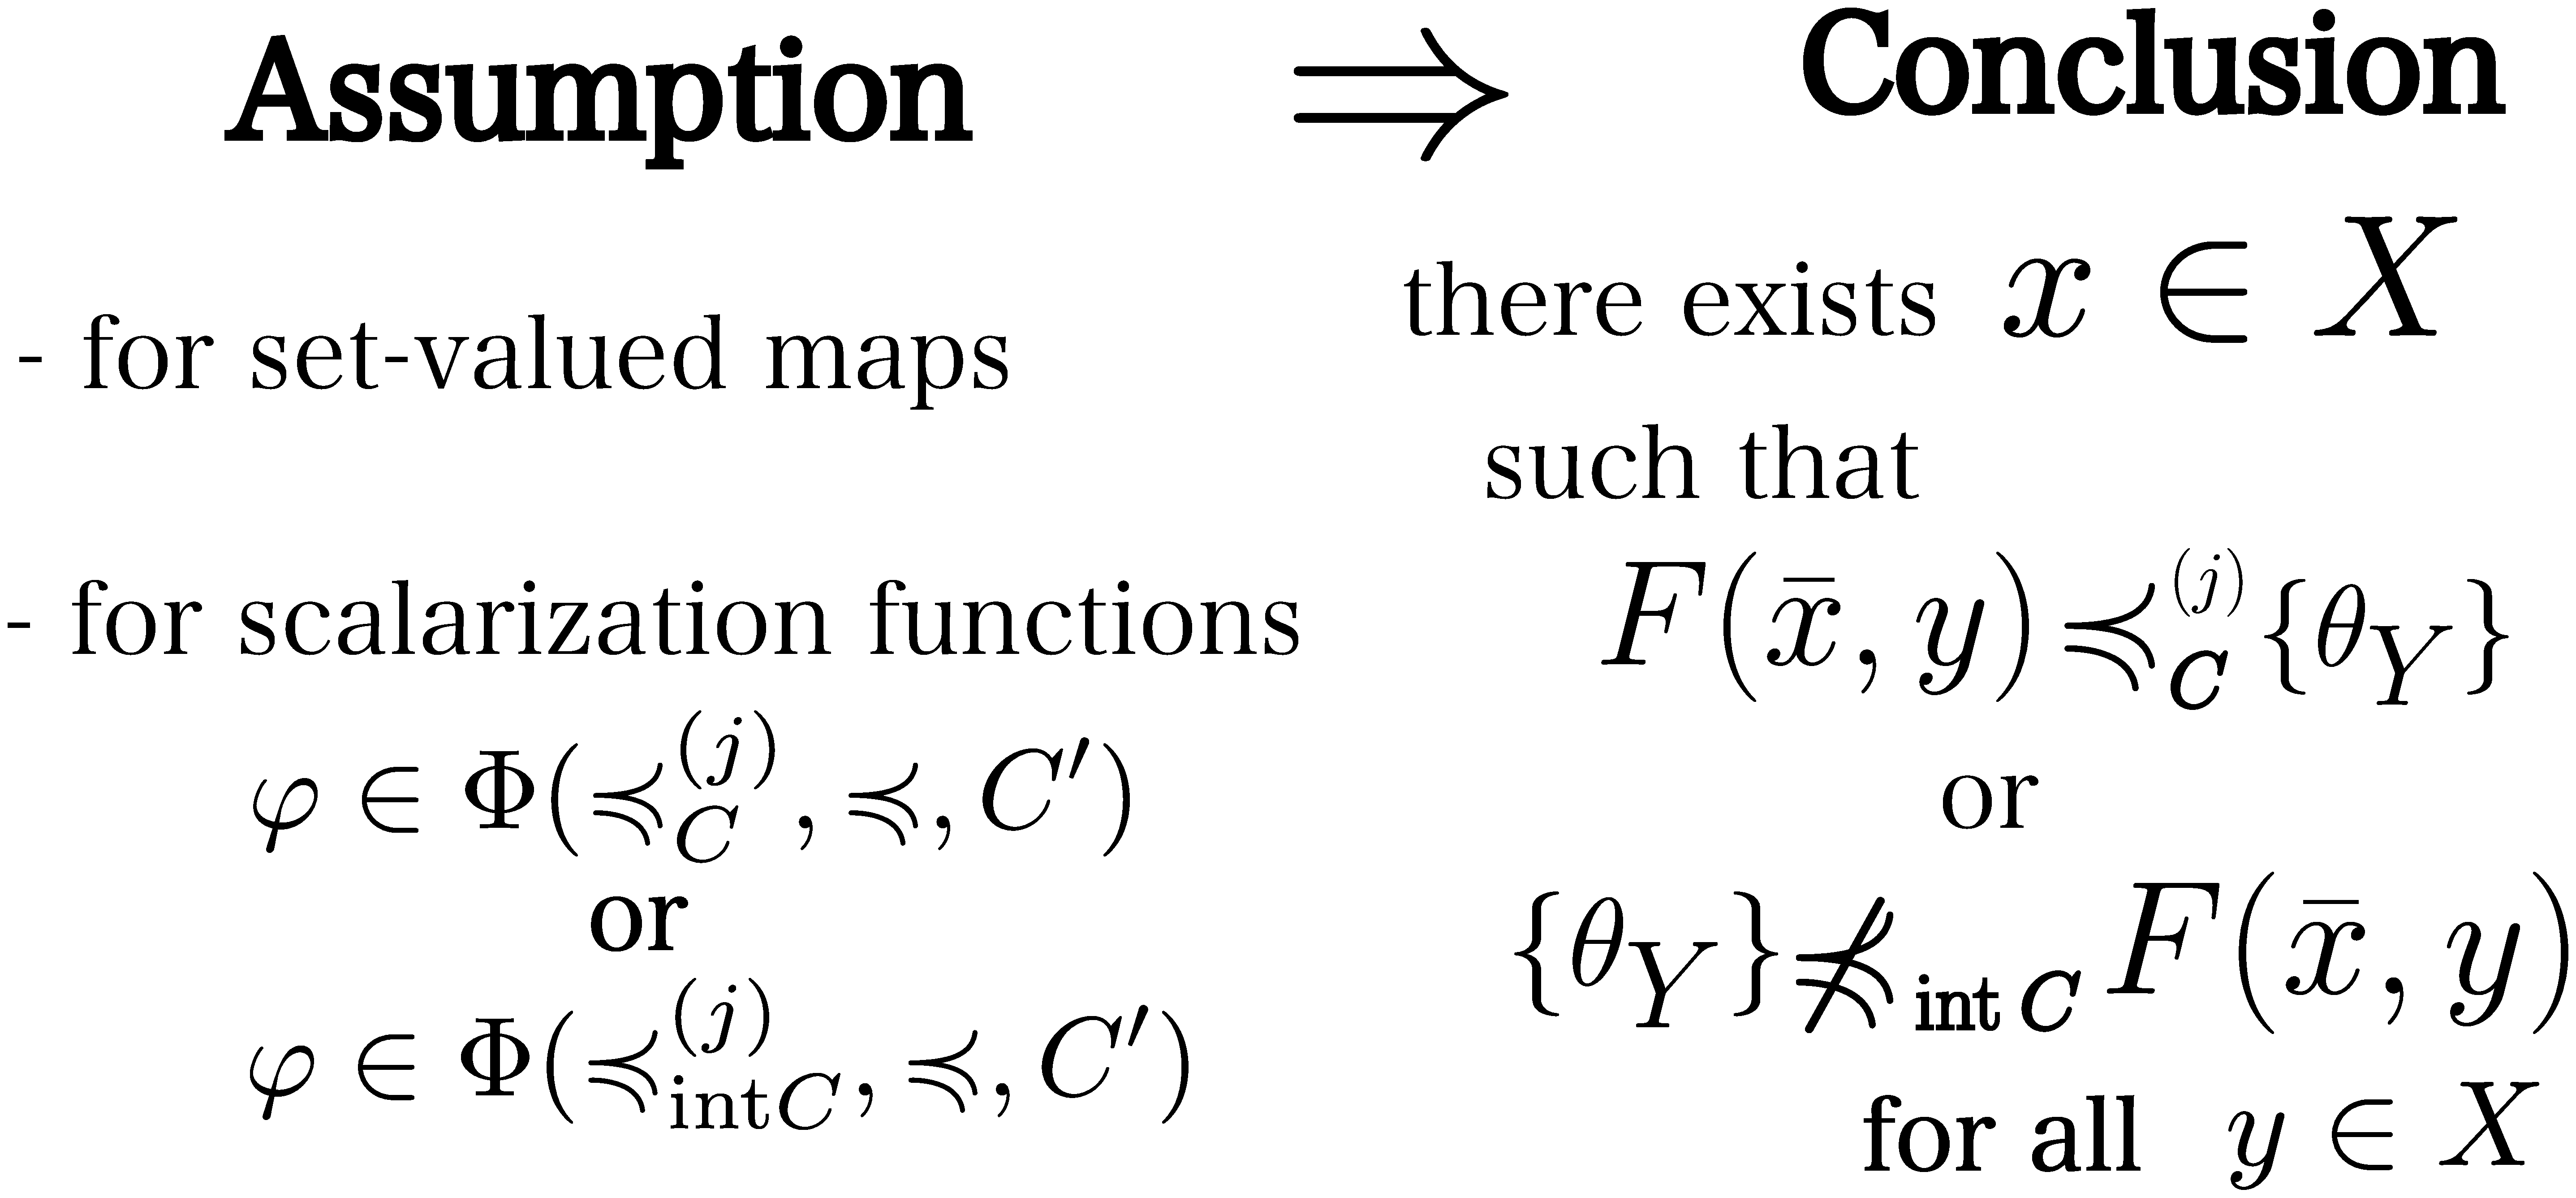
\includegraphics[keepaspectratio, scale=0.13]{figures/eps/main_result_1.eps}
\end{frame}

\begin{frame}{Recap: Set-Valued Fan-Takahashi Inequalities with Set-Relations}
  \centering
  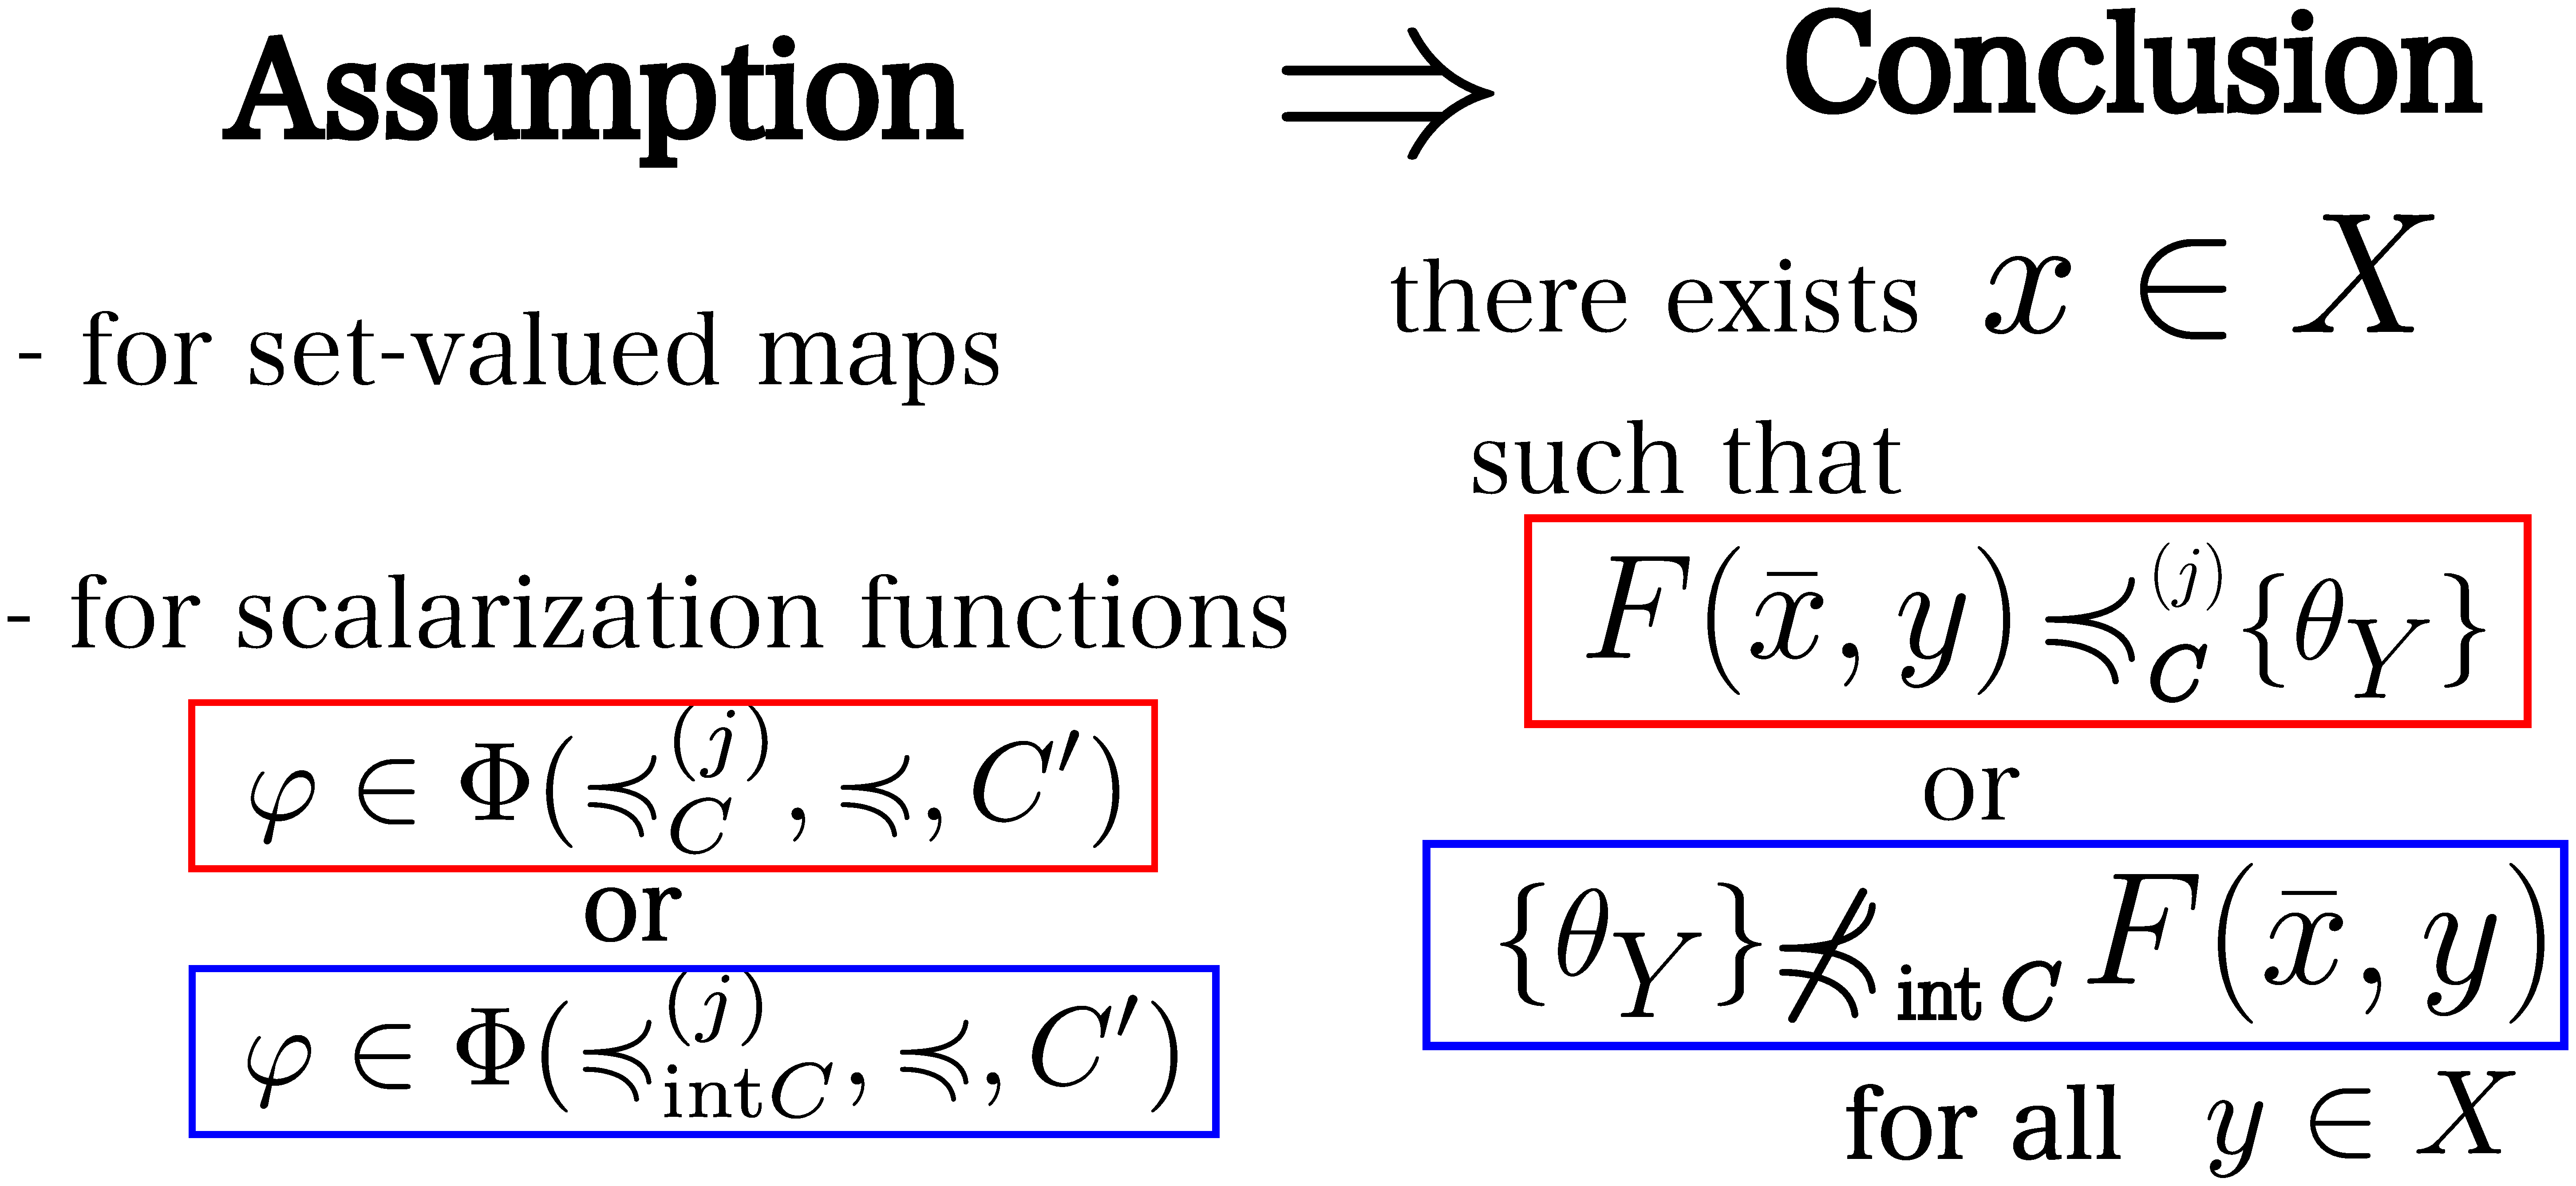
\includegraphics[keepaspectratio, scale=0.13]{figures/eps/main_result_2.eps}
\end{frame}

\begin{frame}{Scalarization Functions (1/2)}
  Let $\varphi: \pow{Y} \to \rnum \cup \{\pm \infty\}$,
  $\setrel{j}{C} (j= 1, 2U, 2L, 3U, 3L, 4)$ set-relations,
  $\preccurlyeq$ a binary relation
  on $\pow{Y}$, and $C' \subset Y$  a convex cone.
  To generalize four types of set-valued minimax inequalities \cite{MR2778674},
  we provide a new class of scalarization functions that satisfy;
  \begin{enumerate}[]
    \item (sc) $\varphi$ is $(\preccurlyeq, C')$-lower semicontinuous;
    \item (qv) $\varphi$ is quasi concave.
  \end{enumerate}
\end{frame}

\begin{frame}{Scalarization Functions (2/2)}
  In addition, we give necessary conditions between values of
  scalarization functions and set-relations as follows;
  \begin{enumerate}[]
    \item (i) $\varphi$ is $(\setrel{j}{C})$-monotone,
    \item (ii) $\varphi (A) \leq 0 \Rightarrow  A \setrel{j}{C} \{\theta_Y\}\quad\text{for any}\:A\in \pow{Y}$,
    \item (i)'$\varphi$ is $(\setrel{j}{\Interior{C}})$-monotone,
    \item (ii)'$\varphi (A) > 0 \Rightarrow  \{\theta_Y\} \setrel{j}{\Interior{C}} A \quad\text{for any}\:A\in \pow{Y}$, and
    \item (iii) $\varphi(\{\theta_{Y}\}) \leq 0$.
  \end{enumerate}
  Supposed that $\varphi$ satisfies conditions (sc) (qv), (i), (ii), and (iii),
  it is written as $\varphi \in \Phi(\setrel{j}{C}, \preccurlyeq, C')$. On the other hand,
  if $\varphi$ satisfies conditions (sc) (qv), (i)', (ii)', and (iii),
  we write the notation as $\varphi \in \Phi(\setrel{j}{\Interior{C}}\:, \preccurlyeq, C')$.
\end{frame}

\begin{frame}{Set-Valued Fan-Takahashi Inequalities with Set-Relations (1/2)}
  \begin{block}{Theorem 1}
    Let $X$ be a nonempty compact convex subset of a Hausdorff topological vector space,
    $Y$ a real topological vector space, $\preccurlyeq$ a binary relation on $\pow{Y}$,
    $C$ a convex cone in $Y$, $C'$ a convex cone in $Y$,
    $\setrel{j}{C} (j= 1, 2U, 2L, 3U, 3L, 4)$ set-relations,
    $\varphi\colon \pow{Y} \to \rnum \cup \{\pm \infty\}$,
    and $F\colon X \times X \to \pow{Y}$.
    For the scaralization function $\varphi \in \Phi(\setrel{j}{C}, \preccurlyeq, C')$,
    if $F$ satisfies the following conditions:
    \begin{enumerate}
      \item $(\varphi \circ F)(x,y) \in \rnum$ for all $x,y \in X$,
      \item for each fixed $y \in X$, $F(\cdot,y)$ is $(\preccurlyeq, C')$-continuous,
      \item for each fixed $x \in X$, $F(x,\cdot)$ is type $(j)$ naturally quasi $C$-concave,
      \item for all $x \in X$, $F(x,x) \setrel{j}{C} \{\theta_Y\}$,
    \end{enumerate}
    then there exists $\bar{x} \in X$ such that $ F(\bar{x},y) \setrel{j}{C} \{\theta_Y\} $ for all $y \in X$.
  \end{block}
\end{frame}

\begin{frame}{Set-Valued Fan-Takahashi Inequalities with Set-Relations (2/2)}
  \begin{block}{Theorem 2}
    Let $X$ be a nonempty compact convex subset of a Hausdorff topological vector space,
    $Y$ a real topological vector space, $\preccurlyeq$ a binary relation on $\pow{Y}$,
    $C$ a convex cone in $Y$, $C'$ a convex cone in $Y$,
    $\setrel{j}{C} (j= 1, 2U, 2L, 3U, 3L, 4)$ set-relations,
    $\varphi\colon \pow{Y} \to \rnum \cup \{\pm \infty\}$,
    and $F\colon X \times X \to \pow{Y}$.
    For the scaralization function $\varphi \in \Phi(\setrel{j}{\Interior{C}}\:, \preccurlyeq, C')$
    if $F$ satisfies the following conditions:
    \begin{enumerate}
      \item $(\varphi \circ F)(x,y) \in \rnum$ for all $x,y \in X$,
      \item for each fixed $y \in X$, $F(\cdot,y)$ is $(\preccurlyeq, C')$-continuous,
      \item for each fixed $x \in X$, $F(x,\cdot)$ is type $(j)$ naturally quasi $C$-concave,
      \item for all $x \in X$, $\{\theta_Y\} \notsetrel{j}{\Interior{C}}\: F(x,x) $,
    \end{enumerate}
    then there exists $\bar{x} \in X$ such that $\{\theta_Y\} \notsetrel{j}{\Interior{C}}\: F(\bar{x},y)$
    for all $y \in X$.
  \end{block}
\end{frame}
% \begin{frame}{Background}
%   - Georgiev and Tanaka \cite{MR1807037} extended \textcolor{orange}{Fan-Takahashi minimax inequality} to the form of set-valued maps.
%   % P. G. Georgiev と T. Tanaka によって集合値への minimax 不等式の拡張が進められた。

%   - Kuwano, Tanaka, and Yamada \cite{MR2778674} constructed the result of \textcolor{orange}{four types of set-valued minimax inequalities
%     with set relations}.
%   % I. Kuwano と T. Tanaka, S. Yamada によって set-relations の比較にに対してスカラー関数を対応させたものの minimax 不等式の拡張が進められた。

%   - \textbf{Our goal is to generalize the result of four types of set-valued minimax inequalities which is not related to the specific set-relations and scalarization functions.}
%   % set-relations の比較に依存しない形、またスカラー化関数がその比較に依存しない形を目指す。
%   \renewcommand{\thefootnote}{\fnsymbol{footnote}}%
%   \footnote[0]{[2] Pando Gr. Georgiev and Tamaki Tanaka. “Vector-valued set-valued variants of
%     Ky Fan's inequality”. In: J. Nonlinear Convex Anal. 1.3 (2000), pp. 245--254.}
%   \footnote[0]{[5] Issei Kuwano, Tamaki Tanaka, and Syuuji Yamada. “Unified scalarization for
%     sets and set-valued Ky Fan minimax inequality”. In: J. Nonlinear Convex Anal.
%     11.3 (2010), pp. 513--525.}
% \end{frame}

% \begin{frame}{Fan-Takahashi Minimax Inequality}
%   \begin{block}{Theorem (Fan-Takahashi \cite{MR399979})} % 高橋先生の論文を引用する形に変更
%     Let $X$ be a nonempty compact convex subset of a Hausdorff topological vector space and $f \colon X \times X \to \RealNumberSet$. If $f$ satisfies
%     the following conditions:
%     \begin{enumerate}
%       \item for each fixed $y \in X$, $f(\cdot,y)$ is lower semicontinuous,
%       \item for each fixed $x \in X$, $f(x,\cdot)$ is quasi concave,
%       \item $f(x,x) \leq 0$ for all $x \in X$,
%     \end{enumerate}
%     then there exists $\bar{x} \in X$ such that $f(\bar{x},y) \leq 0$ for all $y \in X$.
%   \end{block}
% \end{frame}

% \begin{frame}{Ordering and Set-relations}
%   \centering
%   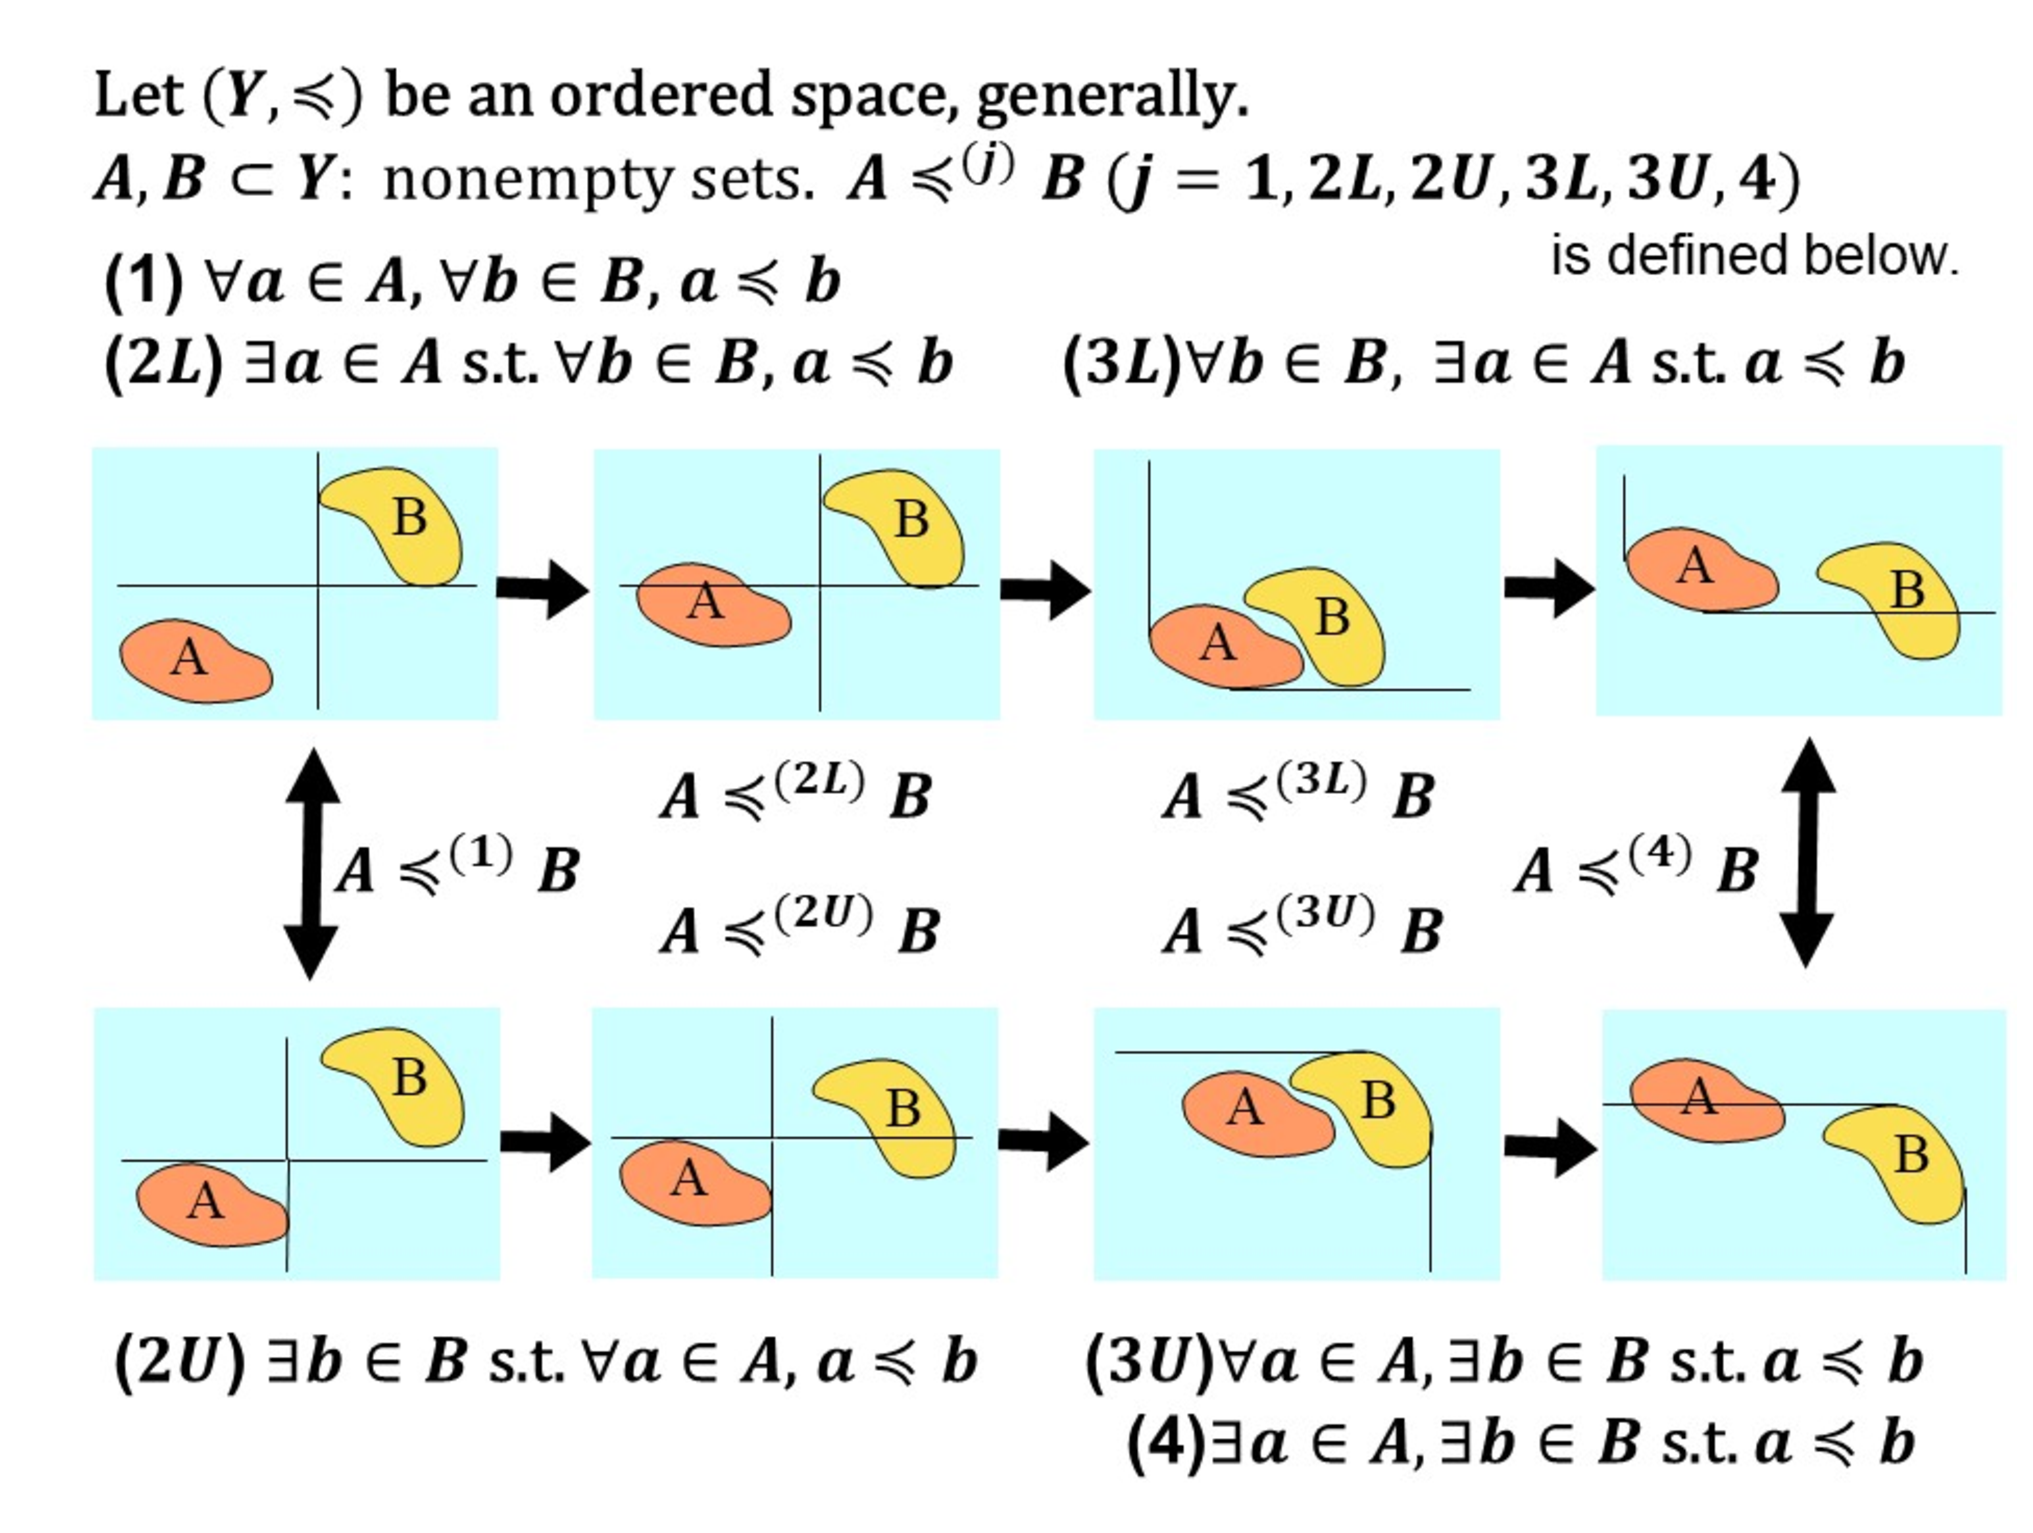
\includegraphics[keepaspectratio, scale=0.28]{figures/eps/set-relations_3.eps}
% \end{frame}

% \begin{frame}{Ordering and Set-relations}
%   \begin{block}{Lemma}
%     Let $Y$ be a real topological vector space, $C$ a convex cone
%     with $\Interior{C} \ne \emptyset$, and $A, \{\theta_Y\} \subset Y$. Then
%     \begin{enumerate}
%       \item $A \setrel{1}{C} \{\theta_Y\} \Leftrightarrow A \setrel{2U}{C} \{\theta_Y\} \Leftrightarrow A \setrel{3U}{C} \{\theta_Y\} \Leftrightarrow A \subset -C$,
%       \item $A \setrel{2L}{C} \{\theta_Y\} \Leftrightarrow A \setrel{3L}{C} \{\theta_Y\} \Leftrightarrow A \setrel{4}{C} \{\theta_Y\} \Leftrightarrow A \cap (-C) \ne \emptyset$,
%       \item $\{\theta_Y\} \notsetrel{1}{\Interior{C}}\:A \Leftrightarrow \{\theta_Y\} \notsetrel{2L}{\Interior{C}}\:A \Leftrightarrow \{\theta_Y\} \notsetrel{3L}{\Interior{C}}\:A \Leftrightarrow A \cap \Interior{C} = \emptyset$,
%       \item $\{\theta_Y\} \notsetrel{2U}{\Interior{C}}\:A \Leftrightarrow \{\theta_Y\} \notsetrel{3U}{\Interior{C}}\:A \Leftrightarrow \{\theta_Y\} \notsetrel{4}{\Interior{C}}\:A \Leftrightarrow A \not\subset \Interior{C}$.
%     \end{enumerate}
%   \end{block}
%   \centering
%   \begin{columns}
%     \begin{column}{0.48\textwidth}
%       \centering
%       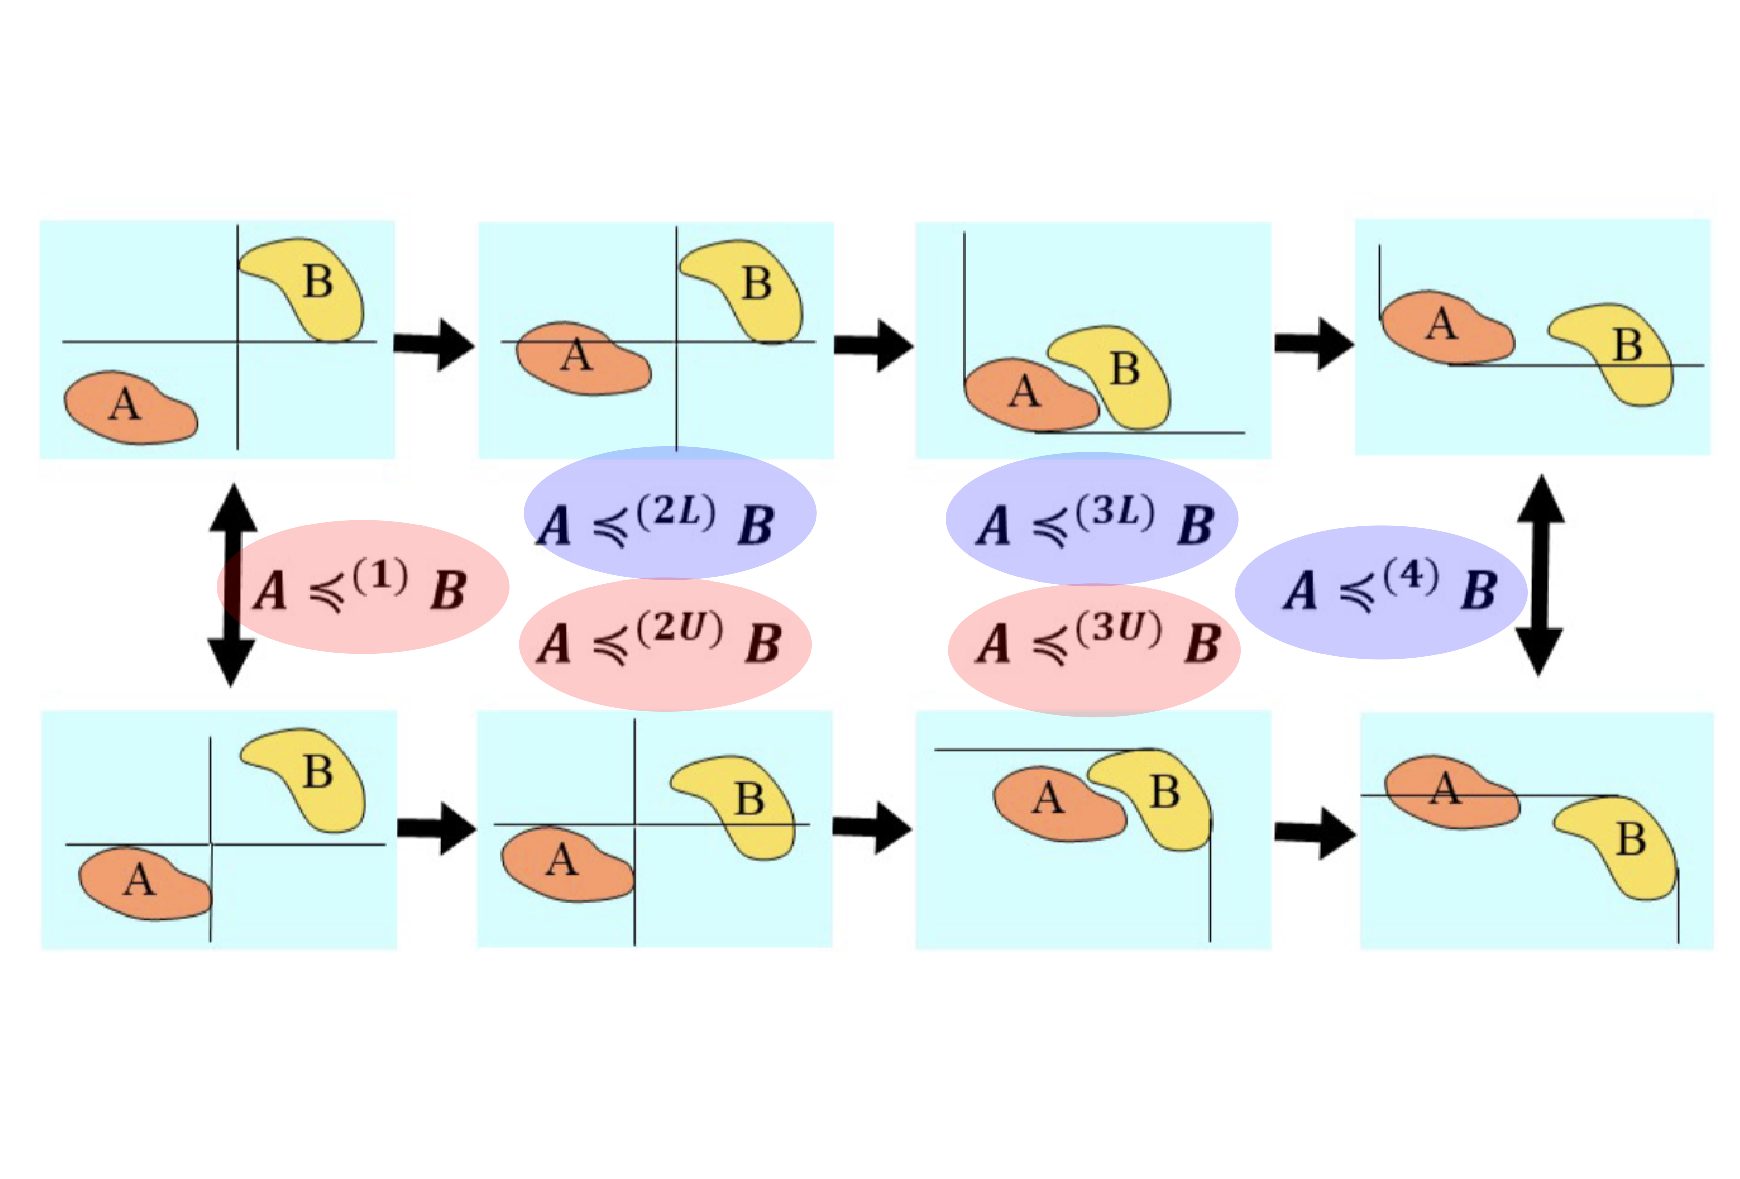
\includegraphics[keepaspectratio, scale=0.18]{figures/eps/case2_set_relations.eps}
%     \end{column}
%     \begin{column}{0.48\textwidth}
%       \centering
%       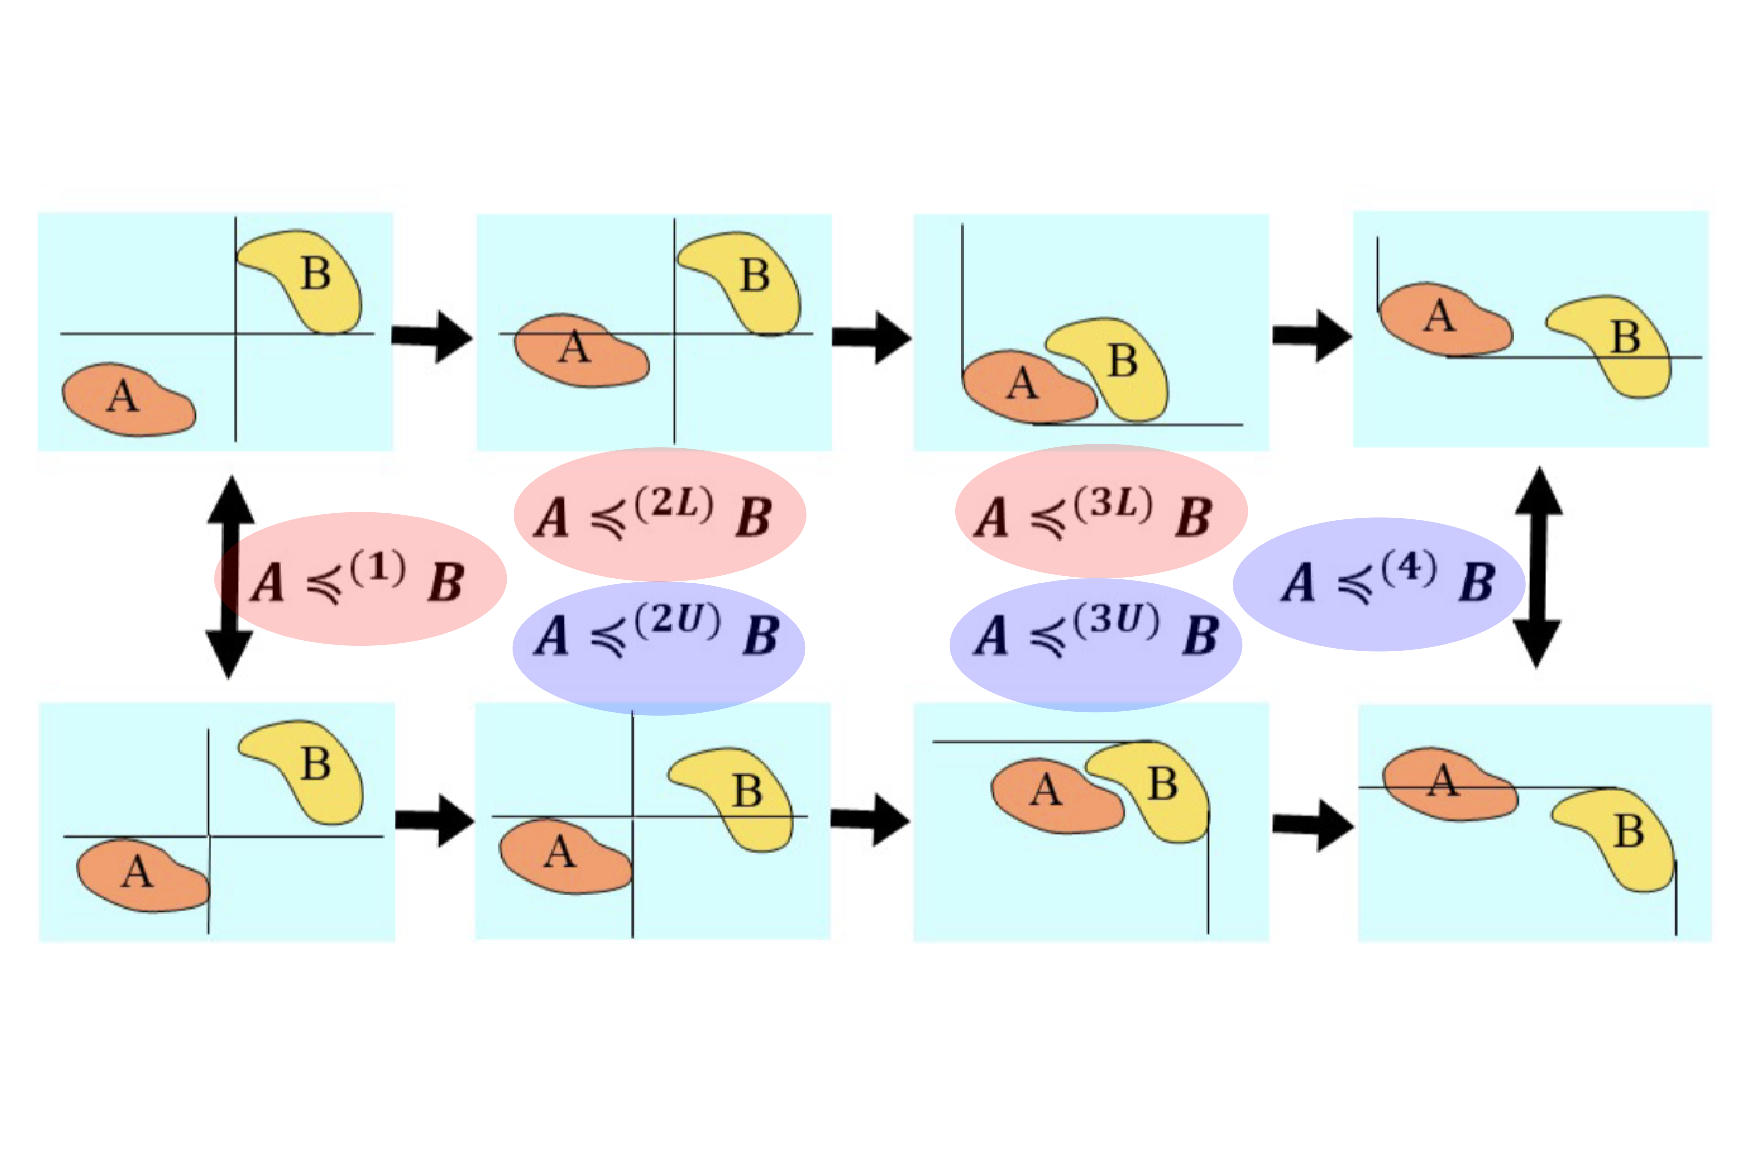
\includegraphics[keepaspectratio, scale=0.18]{figures/eps/case1_set_relations.eps}
%     \end{column}
%   \end{columns}
% \end{frame}

% \begin{frame}{Four types of Set-Valued Minimax Inequalities with Set-relations}
%   Let $f:X \to \RealNumberSet$ and $F:X \to \pow{Y}$.

%   \centering
%   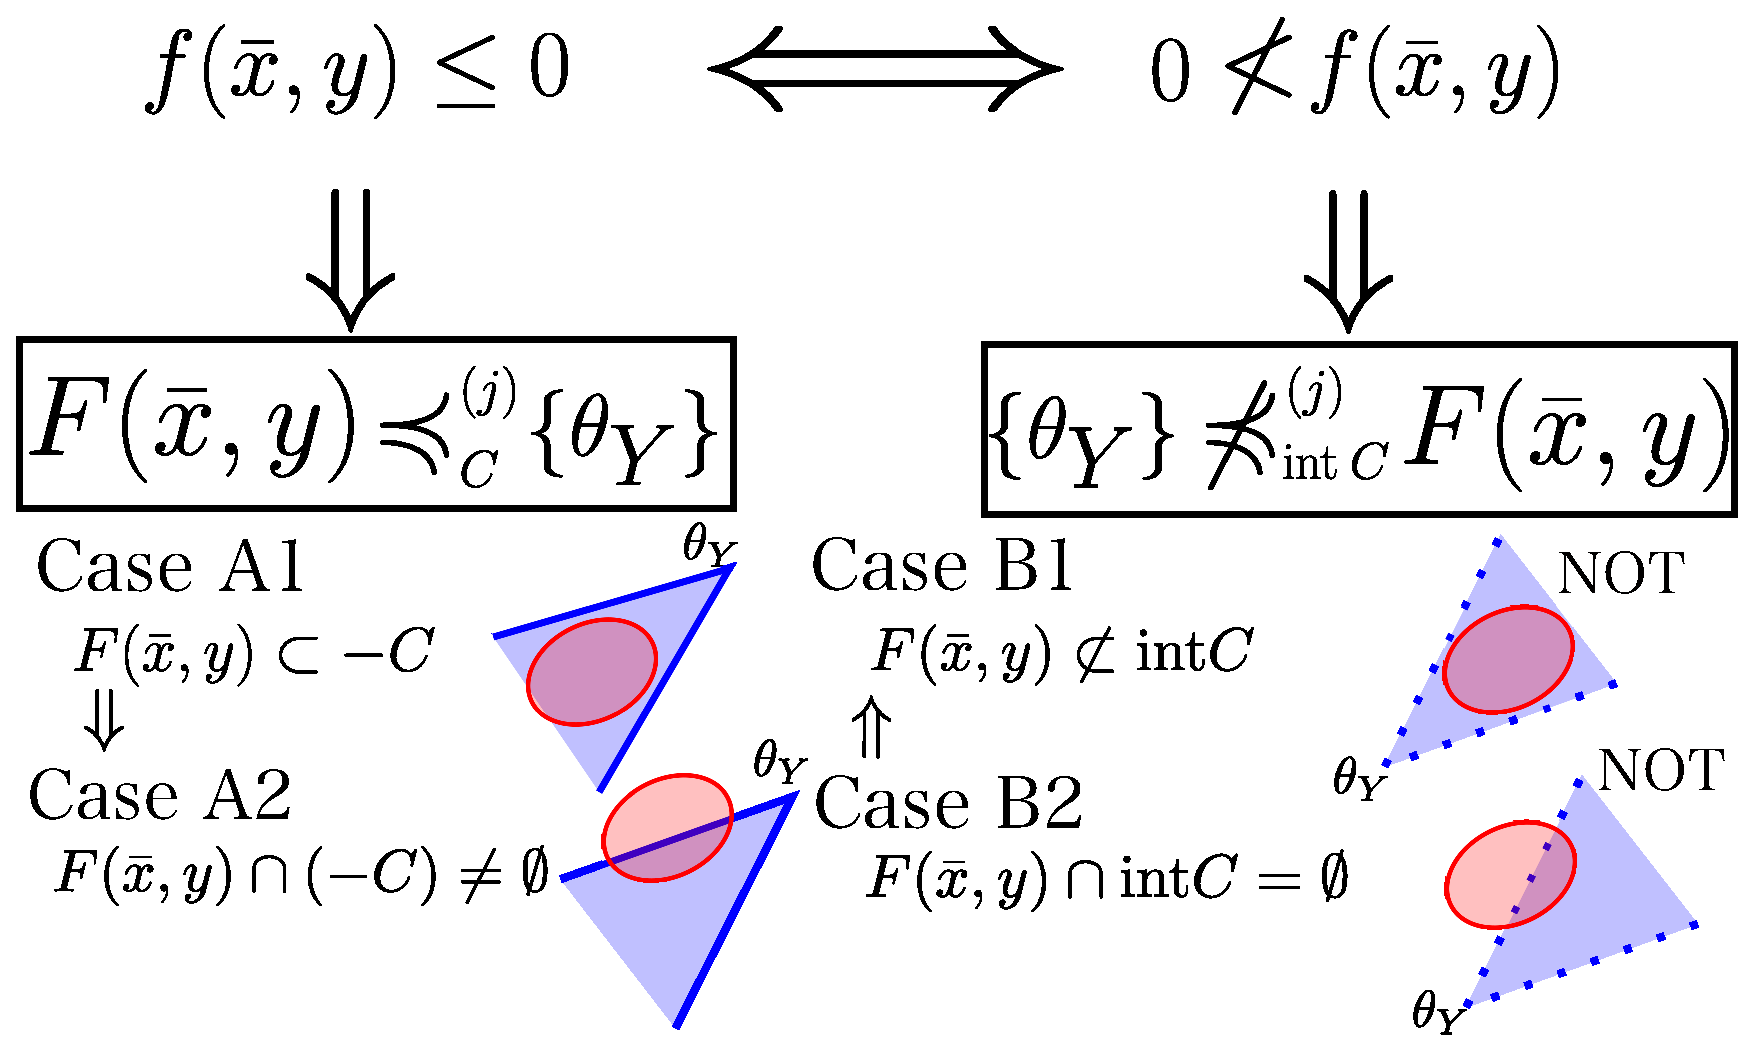
\includegraphics[keepaspectratio, scale=0.35]{figures/eps/4types_set_relations.eps}
% \end{frame}

% \begin{frame}{Four types of Set-Valued Minimax Inequalities with Set-relations}
%   \centering
%   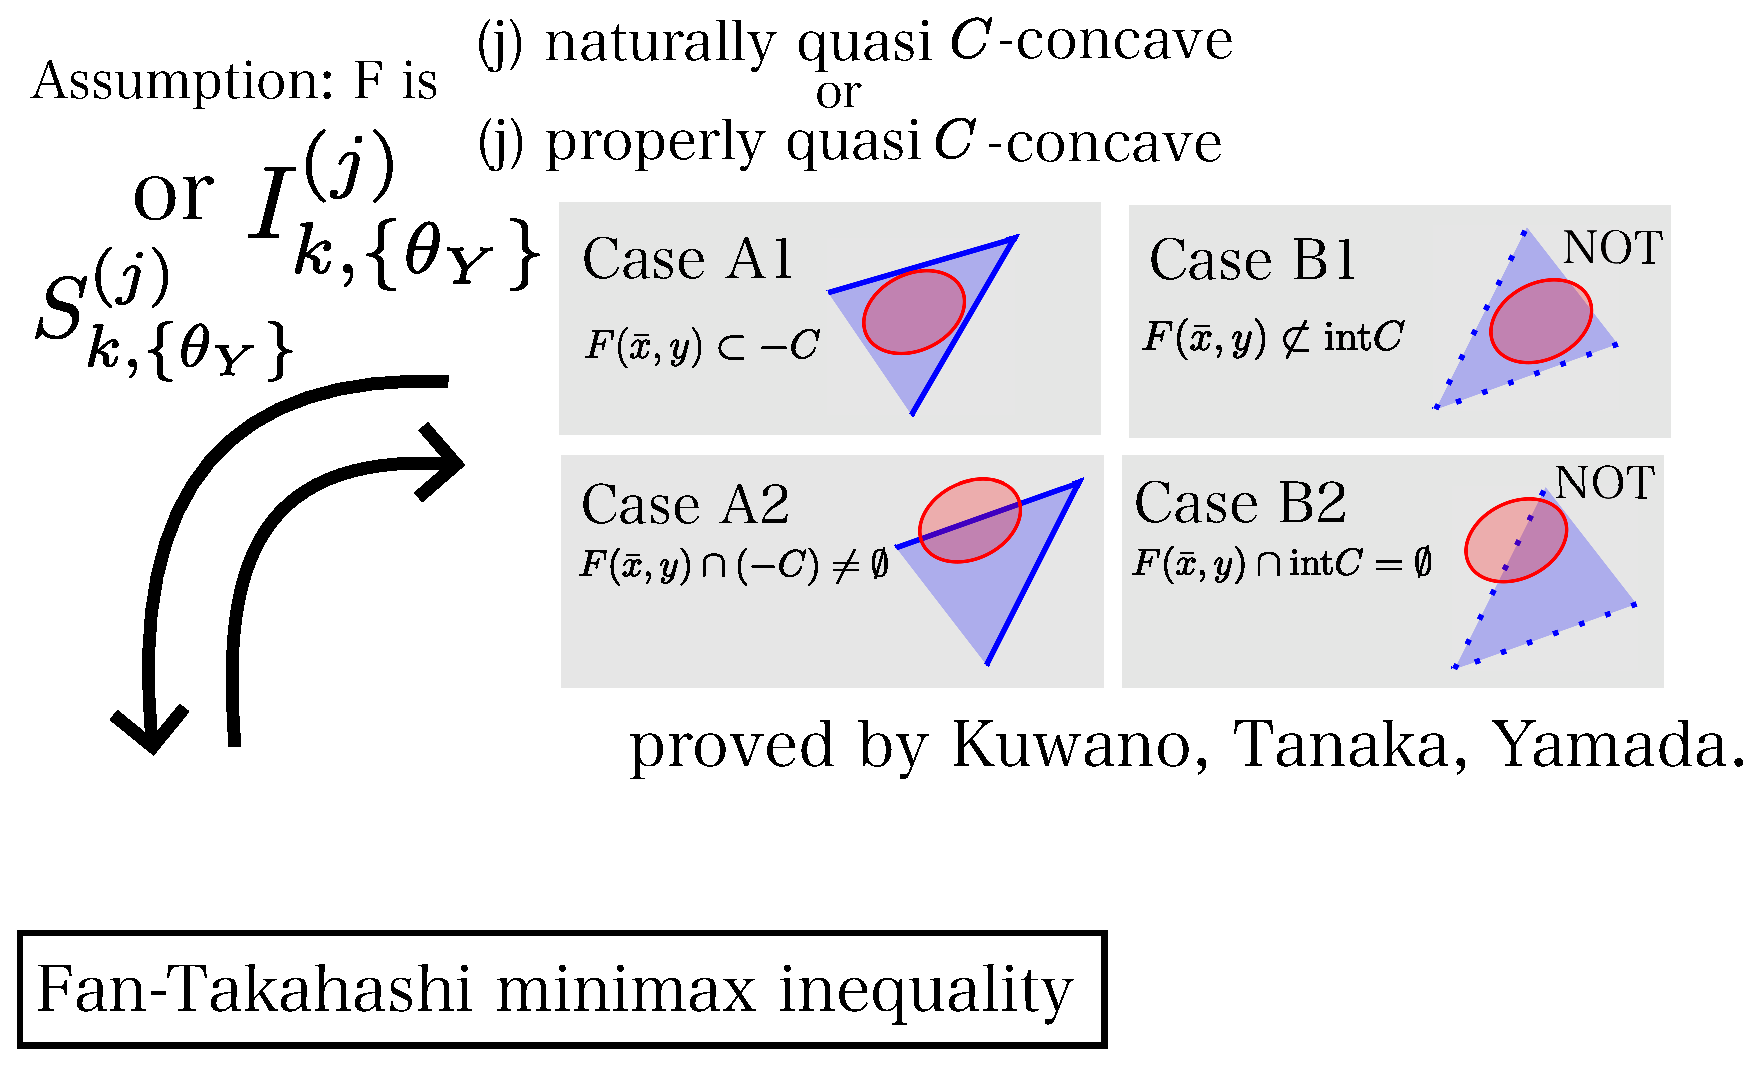
\includegraphics[keepaspectratio, scale=0.38]{figures/eps/kuwano_tanaka_yamada_results.eps}
% \end{frame}

% \begin{frame}{Four types of Set-Valued Minimax Inequalities with Set-relations}
%   \centering
%   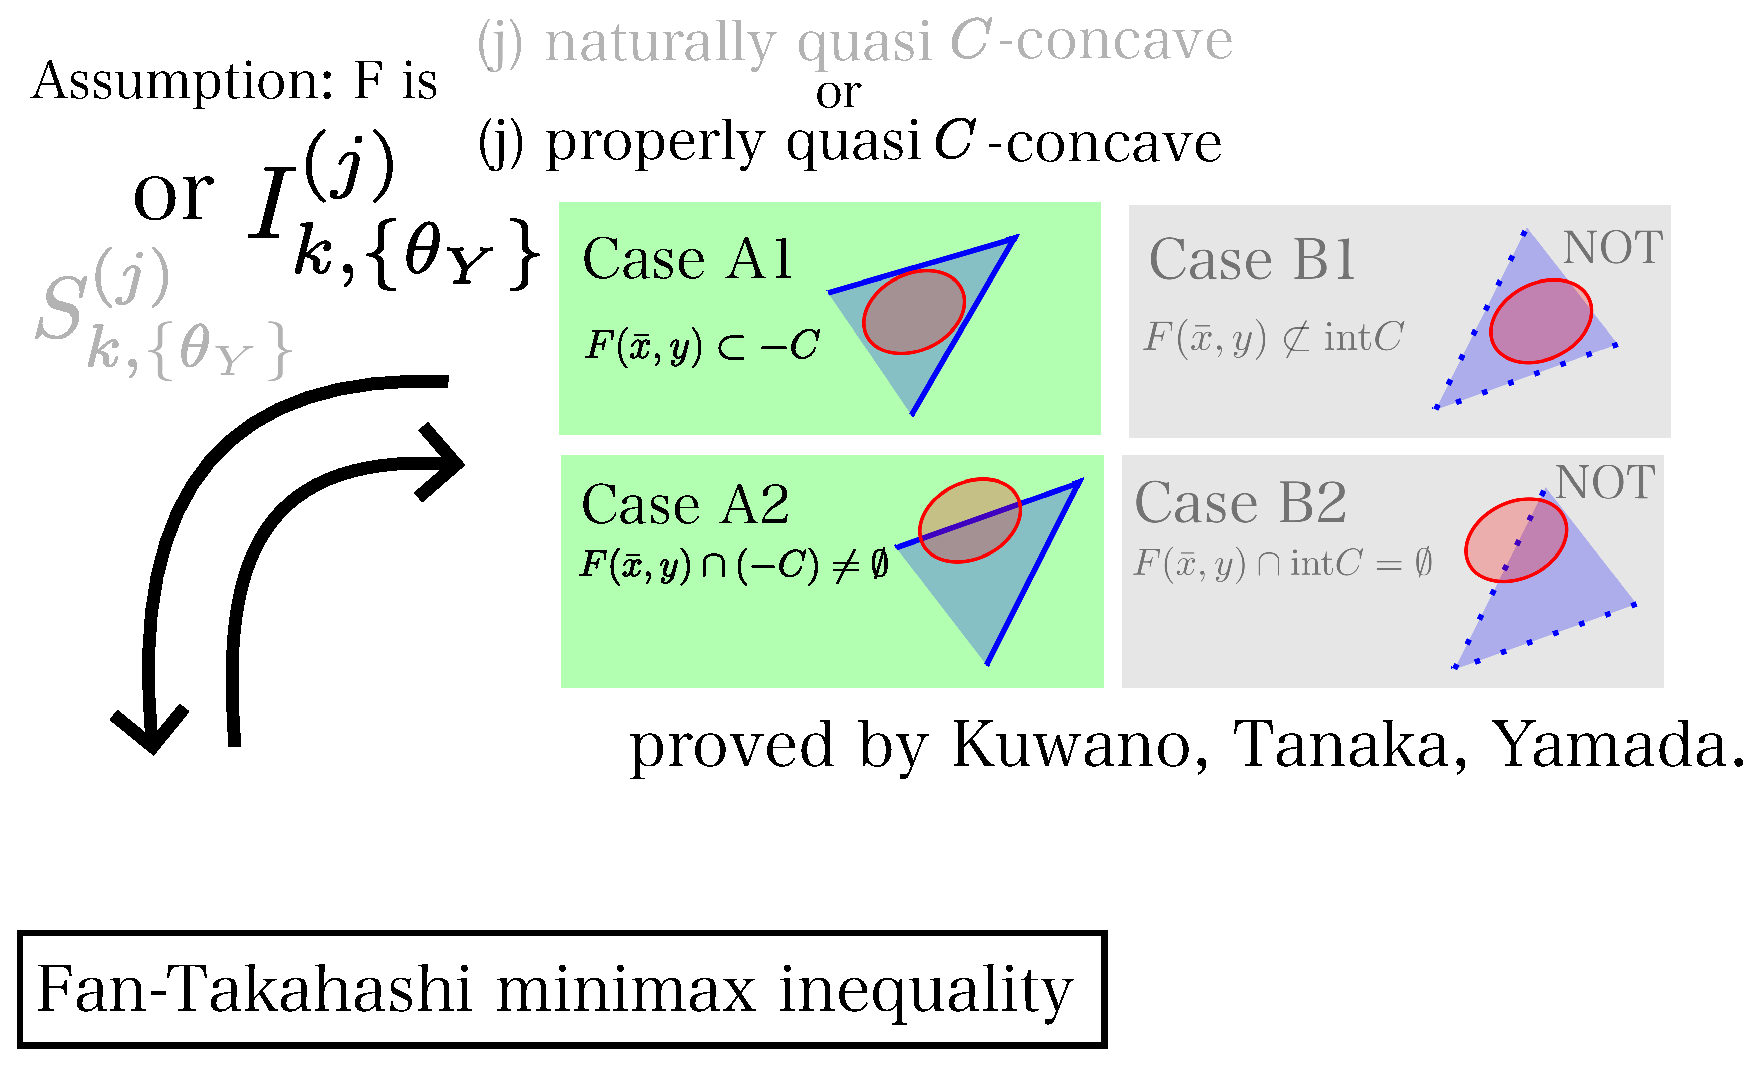
\includegraphics[keepaspectratio, scale=0.38]{figures/eps/kuwano_tanaka_yamada_results_properly.eps}
% \end{frame}

% \begin{frame}{Four types of Set-Valued Minimax Inequalities with Set-relations}
%   \centering
%   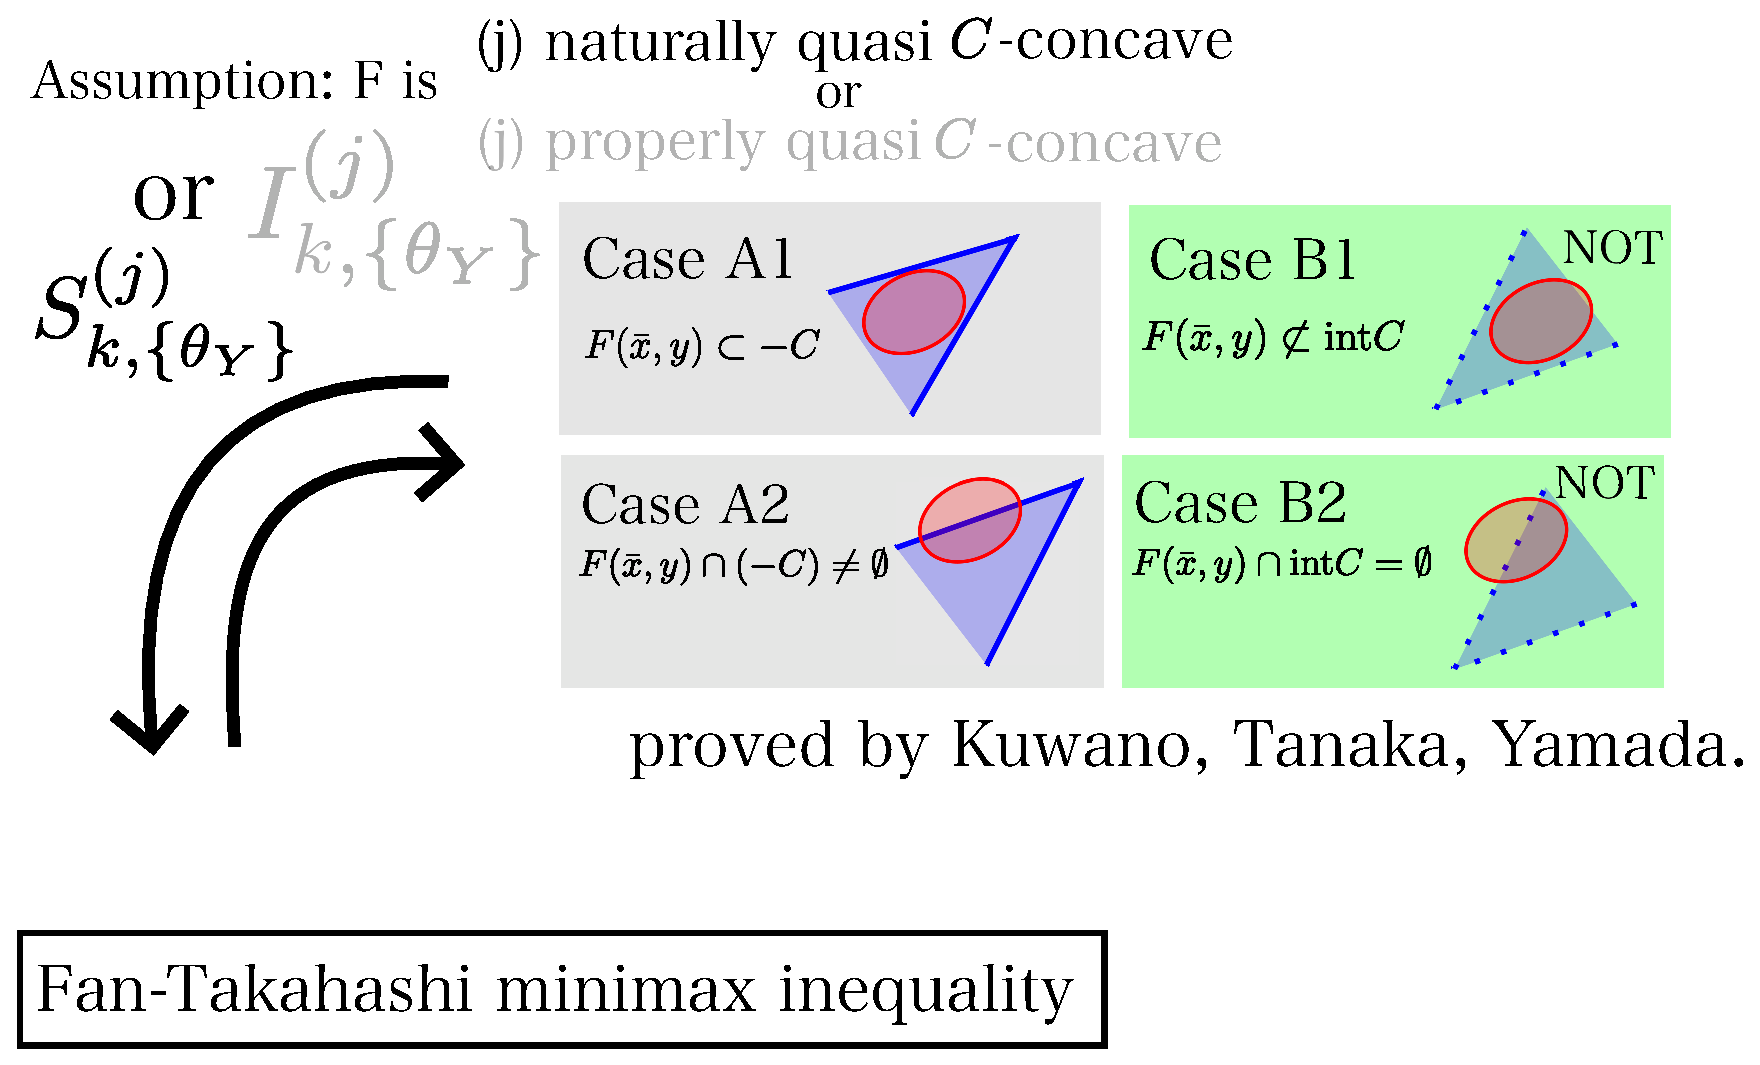
\includegraphics[keepaspectratio, scale=0.38]{figures/eps/kuwano_tanaka_yamada_results_naturally.eps}
% \end{frame}

% \begin{frame}{Our Results}
%   \centering
%   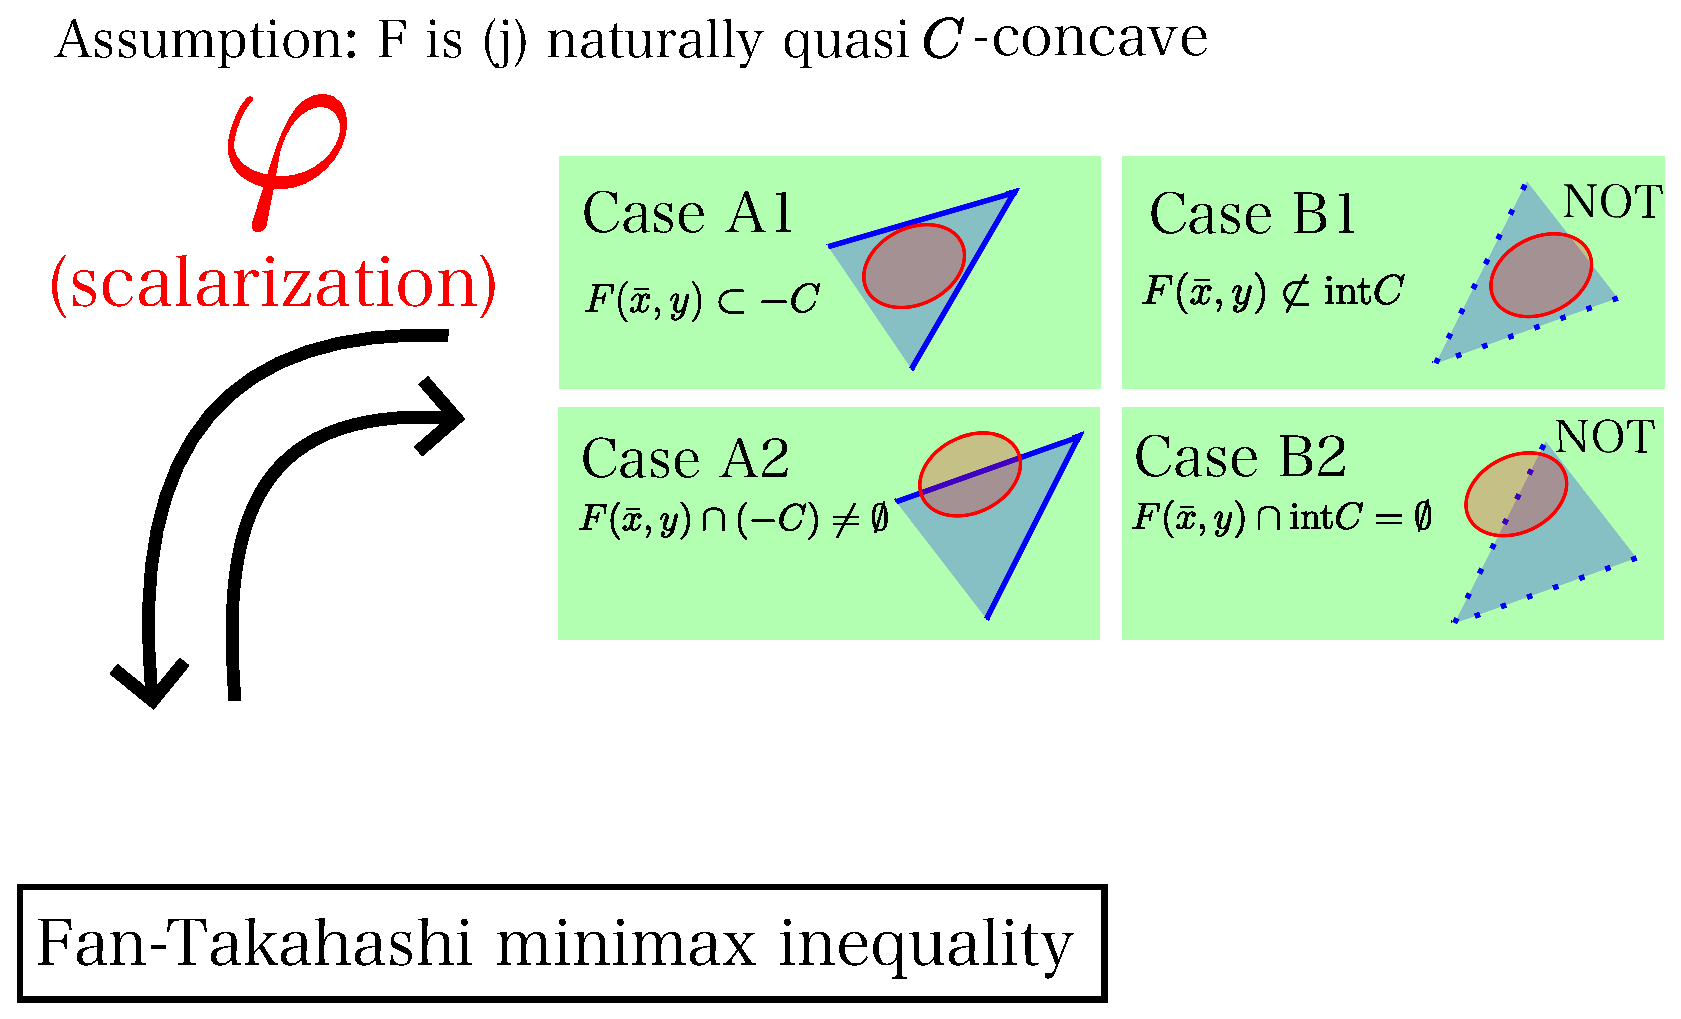
\includegraphics[keepaspectratio, scale=0.38]{figures/eps/iwamoto_tanaka_results.eps}
% \end{frame}

% 5. Examples
% ----------------------------------------------------------------
\section{Scalarization Function: Hiriart-Urruty Oriented Distance}

\begin{frame}{Hiriart-Urruty Oriented Distance}
  \begin{block}{Definition (Hiriart-Urruty Oriented distance) \cite{xu2016new}}
    Let $Y$ be a real normed vector space. For a set $A \subset Y$, let the oriented distance function
    $\Delta_{A} \colon Y \to \RealNumberSet\cup\{\pm \infty\}$ be defined by
    \begin{align*}
      \Delta_{A}(y) \coloneq d_{A} (y) - d_{Y \backslash A}(y),
    \end{align*}
    $ d_{A} (y)= \inf\{\Norm{y - z} \mid z \in A\}$, $d_{\emptyset} (y) \coloneq + \infty$,
    and $\Norm{y}$ denotes the norm of $y$ in $Y$.
  \end{block}
  \begin{block}{Definition (Generalized Hiriart-Urruty Oriented distance) \cite{xu2016new}}
    For the set $A \in Y$, let the functions $\mathcal{D}^{+}_{A} \colon \mathcal{P}(Y) \to \RealNumberSet \cup \{\pm \infty\}$
    and $\mathcal{D}^{-}_{A} \colon \mathcal{P}(Y) \to \RealNumberSet \cup \{\pm \infty\}$ be defined as
    \begin{align*}
      \mathcal{D}^{(1)}_{A}(B) & \coloneq \sup\{\Delta_{A}(b) \mid b \in B\},\: B \in \mathcal{P}(Y),                              \\
      \mathcal{D}^{(2)}_{A}(B) & \coloneq \inf\{-\Delta_{A}(b) \mid b \in B\} = -\mathcal{D}^{(1)}_{A}(B),\: B \in \mathcal{P}(Y).
    \end{align*}x
  \end{block}
\end{frame}

\begin{frame}{Hiriart-Urruty Oriented Distance}
  \begin{exampleblock}{Example}
    Let $Y = \RealNumberSet^{2}$, $A = [0,2] \times [0.2]$, $y_{1} = (1,1)$, and $y_{2} = (3, 3)$. Then,
    \begin{align*}
      \Delta_{A}(y_{1}) & = d_{A}(y_{1}) - d_{Y \backslash A}(y_{1}) = 0 - 1 = -1,        \\
      \Delta_{A}(y_{2}) & = d_{A}(y_{2}) - d_{Y \backslash A}(y_{2}) = \sqrt{2} - 0 = \sqrt{2} .
    \end{align*}
  \end{exampleblock}
  \centering
  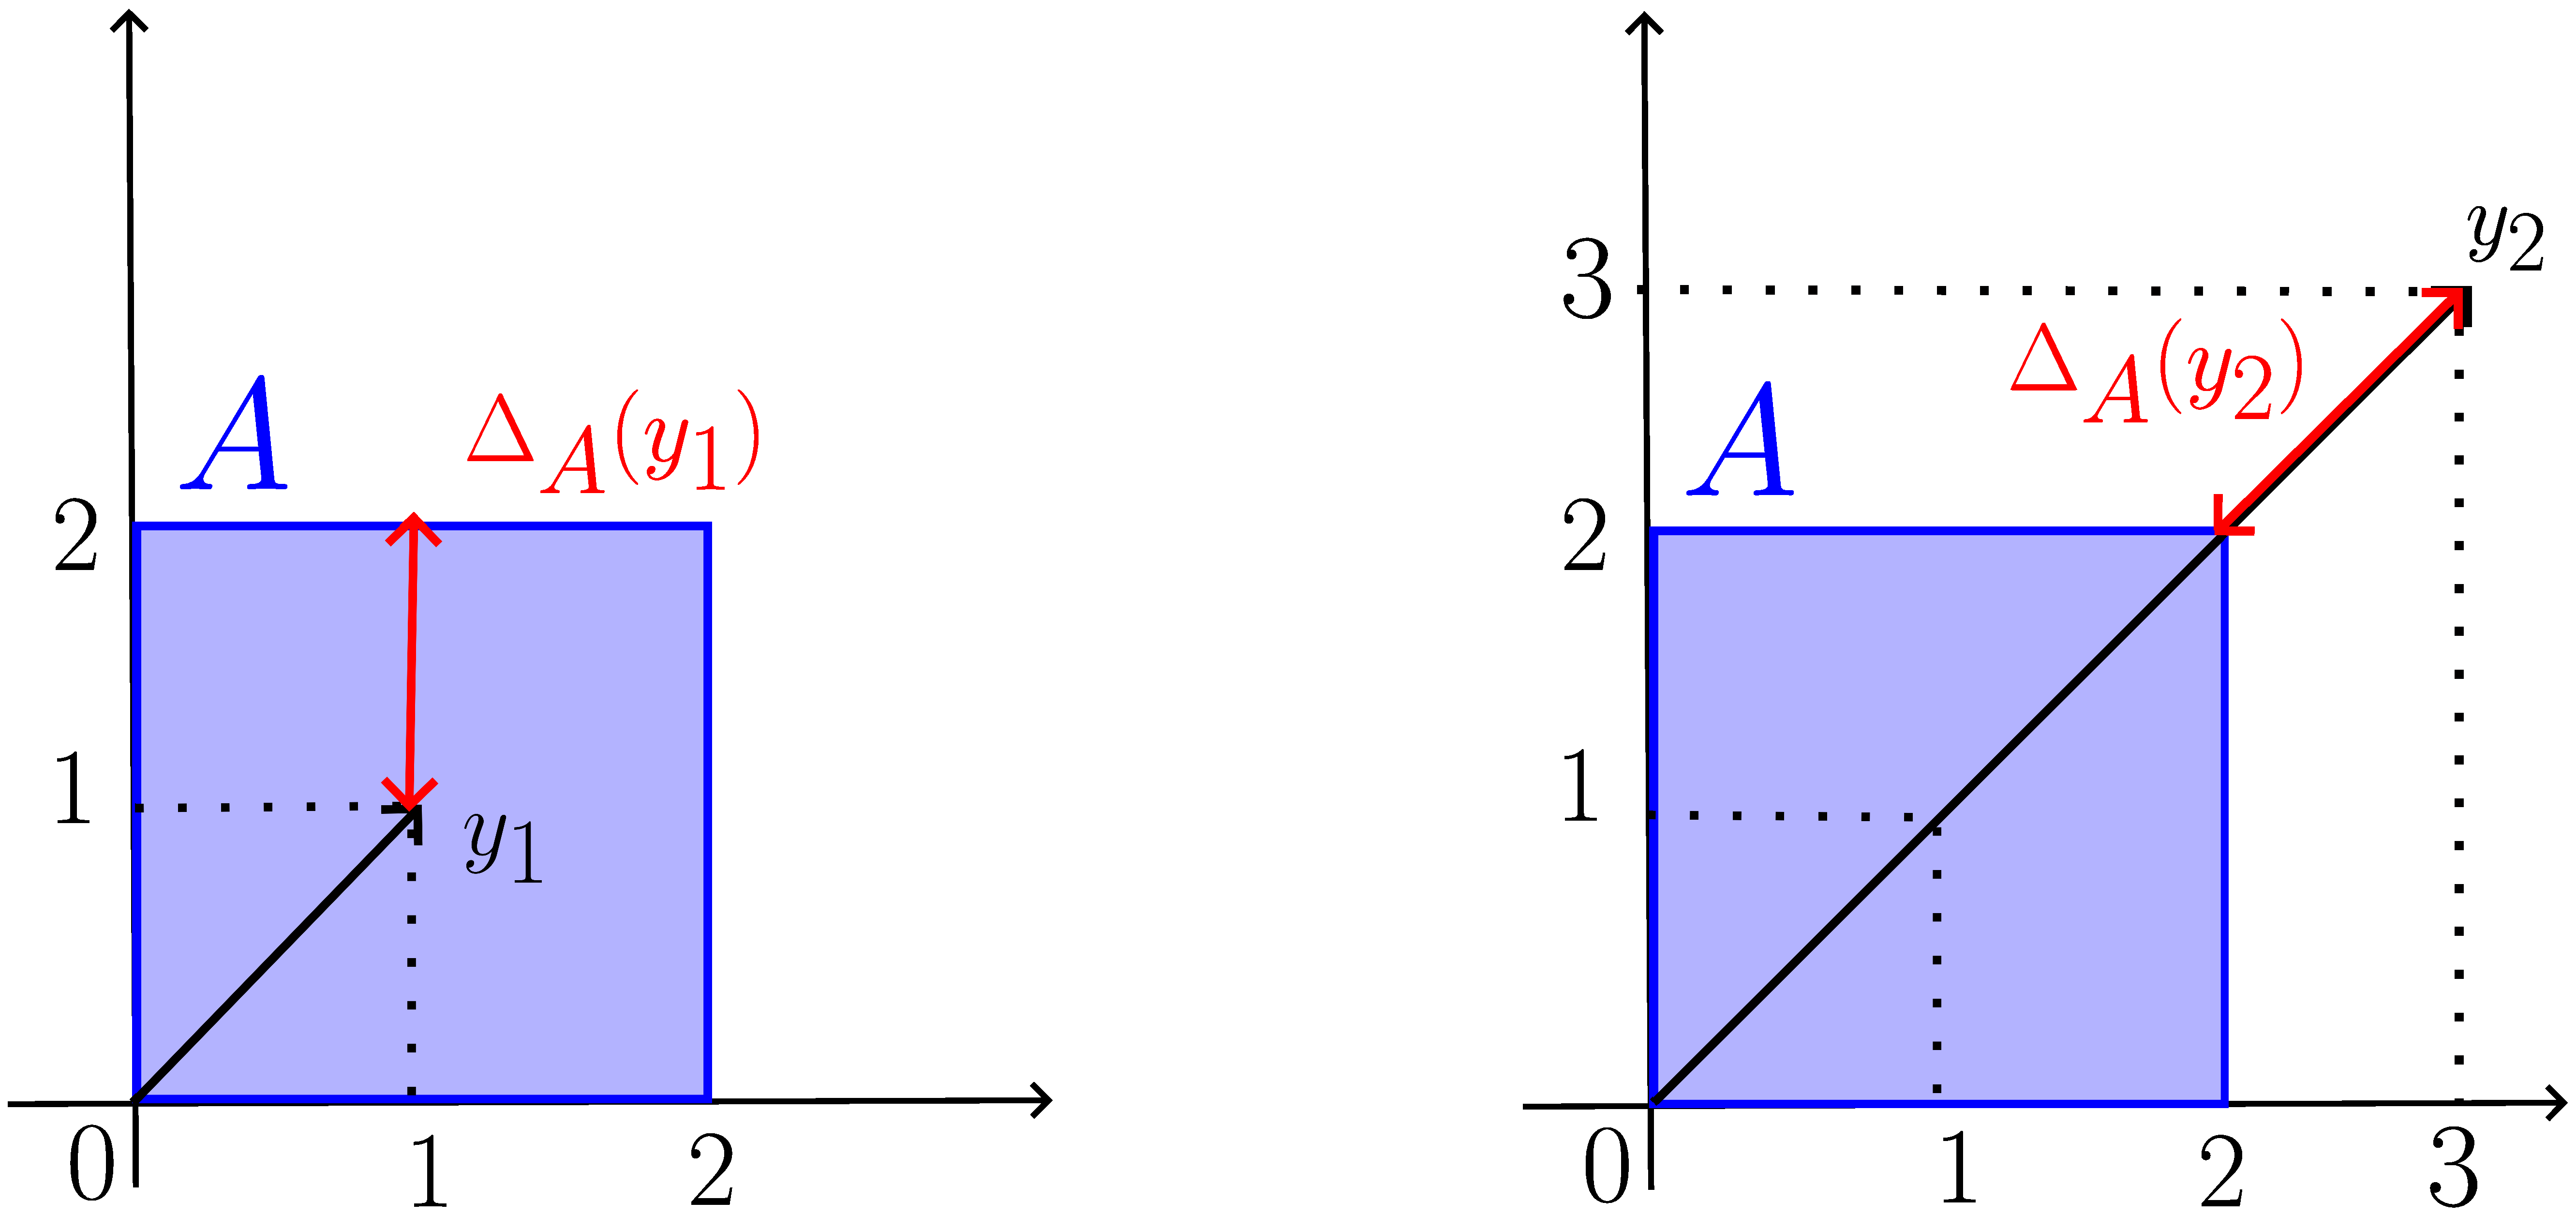
\includegraphics[keepaspectratio, scale=0.10]{figures/eps/hiriart-urruty_distance_example.eps}
\end{frame}

\begin{frame}{Hiriart-Urruty Oriented Distance}
  \begin{block}{Lemma}
    Let $C$ be a proper closed convex cone with $\Interior{C} \ne \emptyset$ in $\hat{Y}$.
    Then, for any set in $\SetForm{B \in \pow{\hat{Y}}}{B \:\text{is $C$-compact}}$,
    $\mathcal{D}^{(2)}_{C}(B) \in \Phi(\setrel{3L}{\Interior{C}}\:, \preccurlyeq_2, C)$.
  \end{block}

  \begin{block}{Proposition}
    Let $X$ be a nonempty compact convex subset of a topological vector space,
    $\hat{Y}$ a real normed vector space, $C$ a proper closed convex cone in $\hat{Y}$ with $\Interior{C} \ne \emptyset$,
    and, $F\colon X \times X \to \pow{\hat{Y}}$.
    If $F$ satisfies the following conditions:
    \begin{enumerate}
      \item $F$ is $C$-compact on $X \times X$,
      \item for each fixed $y \in X$, $F(\cdot,y)$ is $(\preccurlyeq_{2}, C)$-continuous (that is, $C$-upper continuous),
      \item for each fixed $x \in X$, $F(x,\cdot)$ is type $(j)$ naturally quasi $C$-concave,
      \item for all $x \in X$, $\{\theta_{\hat{Y}}\} \notsetrel{3L}{\Interior{C}} F(x,x)$,
    \end{enumerate}
    then there exists $\bar{x} \in X$ such that $\{\theta_{\hat{Y}}\} \notsetrel{3L}{\Interior{C}}\: F(\bar{x},y)$ for all $y \in X$.
  \end{block}
\end{frame}

\begin{frame}{Scalarization Functions (again)}
  In addition, we give necessary conditions between values of
  scalarization functions and set-relations as follows;
  \begin{enumerate}[]
    \item (i) $\varphi$ is $(\setrel{j}{C})$-monotone,
    \item (ii) $\varphi (A) \leq 0 \Rightarrow  A \setrel{j}{C} \{\theta_Y\}\quad\text{for any}\:A\in \pow{Y}$,
    \item (i)'$\varphi$ is $(\setrel{j}{\Interior{C}})$-monotone,
    \item (ii)'$\varphi (A) > 0 \Rightarrow  \{\theta_Y\} \setrel{j}{\Interior{C}} A \quad\text{for any}\:A\in \pow{Y}$, and
    \item (iii) $\varphi(\{\theta_{Y}\}) \leq 0$.
  \end{enumerate}
  Supposed that $\varphi$ satisfies conditions (sc) (qv), (i), (ii), and (iii),
  it is written as $\varphi \in \Phi(\setrel{j}{C}, \preccurlyeq, C')$. On the other hand,
  if $\varphi$ satisfies conditions (sc) (qv), (i)', (ii)', and (iii),
  we write the notation as $\varphi \in \Phi(\setrel{j}{\Interior{C}}\:, \preccurlyeq, C')$.
\end{frame}

\begin{frame}{Scalarization Functions (again)}
  In addition, we give necessary conditions between values of
  scalarization function and set-relations as follows;
  \begin{enumerate}[]
    \item \textcolor{orange}{(i) $\varphi$ is $(\setrel{j}{C})$-monotone,}
    \item \textcolor{orange}{(ii) $\varphi (A) \leq 0 \Rightarrow  A \setrel{j}{C} \{\theta_Y\}\quad\text{for any}\:A\in \pow{Y}$,}
    \item (i)'$\varphi$ is $(\setrel{j}{\Interior{C}})$-monotone,
    \item (ii)'$\varphi (A) > 0 \Rightarrow  \{\theta_Y\} \setrel{j}{\Interior{C}} A \quad\text{for any}\:A\in \pow{Y}$, and
    \item \textcolor{orange}{(iii) $\varphi(\{\theta_{Y}\}) \leq 0$.}
  \end{enumerate}
  Supposed that $\varphi$ satisfies conditions (sc) (qv), (i), (ii), and (iii),
  it is written as $\varphi \in \Phi(\setrel{j}{C}, \preccurlyeq, C')$. On the other hand,
  if $\varphi$ satisfies conditions (sc) (qv), (i)', (ii)', and (iii),
  we write the notation as $\varphi \in \Phi(\setrel{j}{\Interior{C}}\:, \preccurlyeq, C')$.
\end{frame}

\begin{frame}{Characterizing functions}
  \begin{block}{Definition \cite{eichfelder2021optimality}}
    Let $C$ be a convex cone in $Y$ and $f: Y \to \rnum \cup \{\pm \infty\}$.
    We say that $f$ is a characterizing function of the ordering cone $-C$ if
    \begin{equation}
      f(y) \leq 0 \Leftrightarrow y \in -C \quad \text{for all}\: y \in Y. \notag
    \end{equation}
  \end{block}
  \begin{block}{Definition}
    Let $C$ be a convex cone in $Y$ and
    $\setrel{j}{C} (j= 1, 2U, 2L, 3U, 3L, 4)$ set-relations,
    For a scalarization function $\varphi: \pow{Y} \to \rnum \cup \{\pm \infty\}$,
    we consider a class of scalarization functions satisfying
    following three conditions is denoted as $\Phi_0(\setrel{j}{C})$;
    \begin{enumerate}
      \item $\varphi$ is $(\setrel{j}{C})$-monotone,
      \item $\varphi (A) \leq 0 \Rightarrow  A \setrel{j}{C} \{\theta_Y\}\quad\text{for any}\:A\in \pow{Y}$,
      \item $\varphi(\{\theta_{Y}\}) \leq 0$.
    \end{enumerate}
  \end{block}
\end{frame}

\begin{frame}{Characterizing functions}
  \begin{block}{Lemma}
    Let $C$ be a convex cone in $Y$,
    $\setrel{j}{C} (j= 1, 2U, 2L, 3U, 3L, 4)$ set-relations,
    Consider a scalarization function $\varphi \in \Phi_0(\setrel{j}{C})$.
    Then, if we define $f(y) = \varphi (\{y\})$ for any $y \in Y$,
    $f$ is a characterizing function of $-C$.
  \end{block}
  \begin{block}{Lemma}
    Let $C$ be a closed convex cone in $Y$ and $f: Y \to \rnum \cup \{\pm \infty\}$
    a characterizing function of $-C$. Define $\varphi_s : \pow{Y} \to \rnum \cup \{\pm \infty\}$ by
    \begin{equation}
      \varphi_s (A) = \sup_{a \in A} f(a) \quad \text{for all}\: A \in \pow{Y}. \notag
    \end{equation}
    If $f$ satisfies that for all $a, b \in Y$ with $a \bleq{C} b$, $f(a) \leq f(b)$,
    then $\varphi_s$ is an element of $\Phi_0(\setrel{3U}{C})$.
  \end{block}
\end{frame}

% 6. Conclusions
% ----------------------------------------------------------------
\section{Conclusion}

% 6.1
\begin{frame}{Conclusion}
  \begin{itemize}
    \item We can give an example of interior ordering type of set-valued minimax inequalities. 
    However, for ordinary ordering type of set-valued minimax inequalities, these examples are 
    not provided here. As the result between scalarization functions and characterizing functions 
    can be a key element for establishing a new example.
    \item The form of composite functions appear in some fields. Thus, studying
    continuity of set-valued maps, we find other applications except for Fan-Takahashi minimax
    inequality.
  \end{itemize}
\end{frame}

% References
% ----------------------------------------------------------------
\begin{frame}[allowframebreaks]{Reference}
  \printbibliography
\end{frame}

\begin{frame}
  Thank you for your attention!
\end{frame}

\begin{frame}[noframenumbering]{Theme}
  Get the source of this theme and the demo presentation from

  \begin{center}\url{github.com/matze/mtheme}\end{center}

  The theme \emph{itself} is licensed under a
  \href{http://creativecommons.org/licenses/by-sa/4.0/}{Creative Commons
    Attribution-ShareAlike 4.0 International License}.

  \begin{center}\ccbysa\end{center}
\end{frame}

\end{document}
